La tensione di soglia $V_{th}$ di un transistore MOS è definita come quella tensione tra gate e bulk per la quale la popolazione di minoritari all'interfaccia è uguale alla popolazione di maggioritari nel bulk. Questa definizione non può essere usata direttamente per il calcolo della tensione di soglia dei dispositivi, ma si deve passare attraverso l'analisi delle caratteristiche corrente-tensione dei dispositivi. \\
Per l'estrazione del parametro $V_{th}$ esistono numerosi metodi\cite{art2}, la scelta è solitamente dettata da un compromesso che si deve trovare fra complessità della procedura di estrazione della soglia e risultato ottenuto per la specifica applicazione. Per questo studio sono stati presi in considerazione:

\begin{itemize}
  \item \emph{Transconductance Change Method (TCM)};
  \item \emph{Second Difference of the Logarithm of the drain current Minimum method (SDLM)};
  \item \emph{Extrapolation in the Linear Region method (ELR)};
  \item \emph{Ratio Method (RM)}.
\end{itemize}

Per il nostro studio, però, non si è solo interessati al valore in sé della tensione di soglia dei dispositivi, ma anche a come questa varia all'aumentare dell'irraggiamento. Dunque, per ogni metodo non ci si ferma all'estrazione della $V_{th}$ dei dispositivi non irraggiati, ma la si estrae anche dopo ogni step d'irraggiamento e, per ciascuno di questi, si calcola la $\Delta V_{th} = V_{th, Irraggiato}-V_{th, non Irraggiato}$. La scelta di quale metodo usare per le analisi successive viene presa sulla qualità del parametro $\Delta V_{th}$.

\subsection[TCM]{Transconductance Change Method}
Il \emph{Transconductance Change Method, TCM,} definisce la tensione di soglia come la tensione di gate-source $V_{GS}$ corrispondente al picco massimo della derivata della transconduttanza $g_m$ rispetto alla tensione di gate ($\frac{dg_m}{dV_ {GS}}$) ed è valido per bassi valori della tensione $V_{DS}$.\\
Questa definizione si basa sul fatto che, quando il dispositivo passa dalla regione di debole inversione alla regione di forte inversione, la dipendenza della corrente di drain rispetto a $V_{GS}$ passa dall'essere esponenziale all'essere lineare.
La transconduttanza è definita come la derivata prima della corrente $I_D$ rispetto alla tensione $V_{GS}$, dunque la derivata della $g_m$ corrisponde alla derivata seconda di $I_D$. Per questo motivo, il massimo di $\frac{dg_m}{dV_{GS}}$ coincide con la tensione alla quale il grafico della corrente passa dalla forma esponenziale a quella lineare. Se $V_{DS}$ è piccola, la tensione per la quale la $g_m$ è massima è molto simile a $V_{th}$.

\begin{figure}[h!]
  \centering
  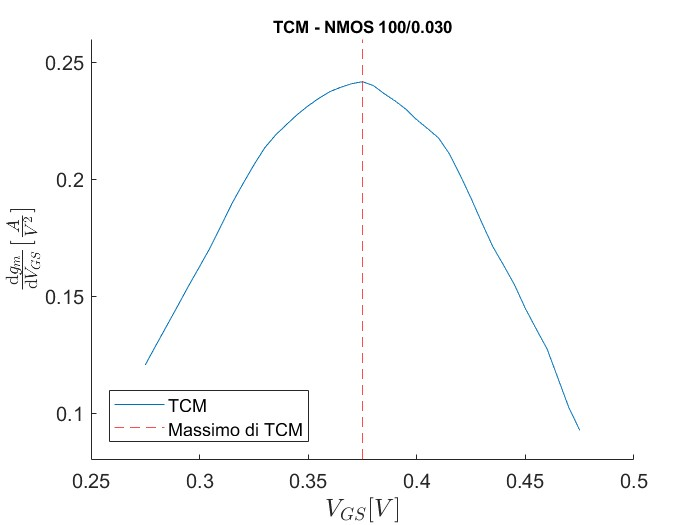
\includegraphics[width=0.49\textwidth]{./capitolo2/VTH/TCM/TCM-N4-100-30-NoFit}
  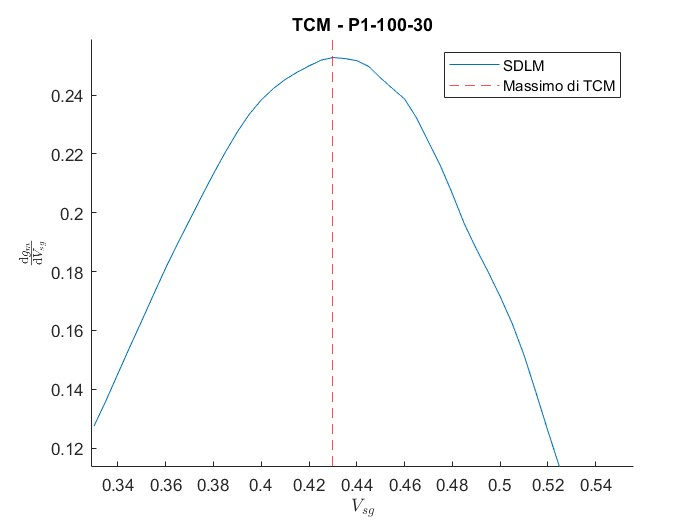
\includegraphics[width=0.49\textwidth]{./capitolo2/VTH/TCM/TCM-P1-100-30-NoFit}
  \caption[Applicazione TCM senza fit polinomiale]{Esempio di \emph{TCM} usato su un dispositivo NMOS e un dispositivo PMOS di dimensioni 100-0.030 a $V_{DS} = 150 mV$}
\end{figure}

Per calcolare il \emph{TCM} si deve trovare il massimo di una funzione, ovvero calcolarne la derivata prima. In questo caso si tratta in realtà di una derivata seconda, essendo già $g_m$ calcolato con una derivata. Il calcolo della derivata non è effettuato su una funzione continua ma su dati misurati con uno step di $5mV$ di $V_{GS}$. Questo fa si che la derivata prima e in modo maggiore la derivata seconda, siano affette da vere e proprie variazioni repentine dovute alla natura granulare dei dati e non da fenomeni fisici. È quindi necessario rendere la funzione studiata meno dipendente da questo effetto. Inoltre, come detto in precedenza, la risoluzione con la quale sono state fatte le misure della corrente di drain è $5mV$ (di $V_{GS}$). Pertanto, con questo metodo si estrarrebbe una soglia che avrebbe una risoluzione di $5mV$, del tutto inaccettabile in quanto sarebbe maggiore delle variazioni di soglia che potrebbero essere indotte dall'irraggiamento.
Per far fronte a questi due problemi, si è scelto di non tenere conto del massimo direttamente ottenuto dallo studio di $\frac{dg_m}{dV_{GS}}$ ottenuto dai valori delle misure, ma d'interpolare prima i punti del grafico con una funzione polinomiale e, di ricavare il valore di soglia da questa funzione.

\begin{figure}[H]
  \centering
  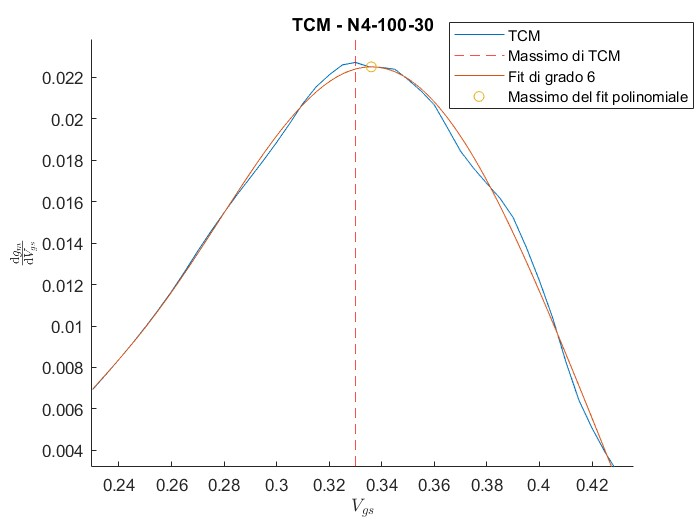
\includegraphics[width=0.49\textwidth]{./capitolo2/VTH/TCM/TCM-N4-100-30}
  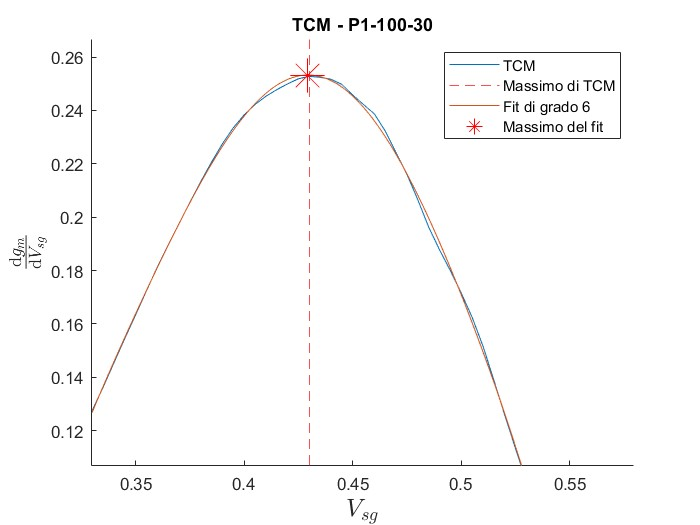
\includegraphics[width=0.49\textwidth]{./capitolo2/VTH/TCM/TCM-P1-100-30}
  \caption[Applicazione TCM con fit polinomiale di sesto grado]{Esempio di \emph{TCM} con fit polinomiale usato su un dispositivo NMOS e un dispositivo PMOS di dimensioni 100-0.030 a $V_{DS} = 150 mV$}
\end{figure}

Lo studio del fit polinomiale risolve il problema della bassa risoluzione di misura, ma presenta una potenziale nuovo problema: il valore della $V_{th}$ calcolata potrebbe variare significativamente al variare del grado della funzione polinomiale interpolante. Per capire l'effetto del grado della funzione interpolante sul valore di tensione di soglia estratto, si sono effettuate le estrazioni considerando i gradi 2, 4, 6 e 8 e si sono studiati i risultati ottenuti. Lo studio si è effettuato su dispositivi PMOS. Una volta scelto il valore del grado della funzione, lo stesso grado sarà utilizzato anche per l'estrazione della tensione di soglia degli NMOS.

\begin{table}[t]
  \renewcommand{\arraystretch}{1.3}
  \centering
  \begin{tabular}{m{2.1cm} m{2cm} m{2cm} m{2cm} m{2cm}}
    \toprule
    \multirow{2}{*}{Dispositivo} & \multicolumn{4}{c}{$V_{th} [mV] \text{ con interpolante di grado:}$}                         \\
    \cmidrule{2-5}
                                 & 2                                                                    & 4     & 6     & 8     \\
    \midrule
    100 - 0.030                  & 426.9                                                                & 429.4 & 429.4 & 430.8 \\
    \hline
    100 - 0.060                  & 467.6                                                                & 469.5 & 469.3 & 468.9 \\
    \hline
    200 - 0.030                  & 397.8                                                                & 399.7 & 399.3 & 399.8 \\
    \hline
    200 - 0.060                  & 452.2                                                                & 454.1 & 453.5 & 453.5 \\
    \hline
    200 - 0.180                  & 495.6                                                                & 495.6 & 495.3 & 495.5 \\
    \hline
    600 - 0.030                  & 383.0                                                                & 387.4 & 385.9 & 386.2 \\
    \hline
    600 - 0.060                  & 431.1                                                                & 434.3 & 434.7 & 435.6 \\
    \hline
    600 - 0.180                  & 478.5                                                                & 480.8 & 480.6 & 480.0 \\

    \bottomrule
  \end{tabular}
  \caption[Confronto $V_{th}$ al variare del grado del fit polinomiale con il metodo TCM]{Confronto dei valori di $V_{th}$ dei dispositivi PMOS ottenuti con \emph{TCM} con fit polinomiale di diversi gradi}
  \label{tab:GradiTCM}
\end{table}

Osservando i valori nella tabella \ref{tab:GradiTCM}, si può notare che la tensione di soglia ottenuta non varia molto nel caso dei fit fatti con polinomiali di grado 4, 6 e 8: è raro che la differenza tra questi valori superi $1 mV$. Non si può dire la stessa cosa per le $V_{th}$ calcolate con fit di grado 2: in questo caso la funzione interpolante ha un grado troppo basso per seguire in modo coerente la curva $\frac{dg_m}{dV_{GS}}$ e quindi il massimo risulta essere molto diverso da quelli calcolati con fit di grado maggiore. Dunque, al fine di fittare al meglio la curva, si è scelto un fit polinomiale di grado 6. In Tabella \ref{tab:VthTCMN} e \ref{tab:VthTCMP} sono riportati i risultati ottenuti con il metodo \emph{TCM} e fit polinomiale di grado 6 su dispositivi PMOS\footnote{Per i PMOS viene indicata la $|V_{th}|$ } e NMOS pre e post irraggiamento.
Mentre nelle tabelle \ref{tab:deltaVthTCMN}, \ref{tab:deltaVthTCMP} e nei grafici a figura \ref{fig:deltaVthTCM} vengono riportati i valori della $\Delta V_{th}$ in funzione della dose assorbita\footnote{La $\Delta V_{th} $ riportata per i PMOS è da intendersi come: $\Delta V_{th} = |V_{th_{post}}| - |V_{th_{pre}}|$}.


\begin{center}
  \begin{table}[h!]
    \renewcommand{\arraystretch}{1.3}
    \resizebox{\textwidth}{!}{%
      \begin{tabular}{c c c c c c c c c c }
        \toprule
        \multirow{2}{*}{Dispositivo} & \multicolumn{9}{c}{$V_{th} [mV] $}                                                                                          \\
        \cmidrule{2-10}
                                     & pre                                & $5Mrad$ & $50Mrad$ & $100Mrad$ & $200Mrad$ & $600Mrad$ & $1Grad$ & $3Grad$ & annealing \\
        \midrule
        100 - 0.030                  & 371.3                              & 370.6   & 361.0    & 380.6     & 378.7     & 375.1     & 371.1   & 367.1   & 372.4     \\
        \hline
        100 - 0.060                  & 405.0                              & 399.9   & 390.0    & 419.8     & 418.8     & 414.0     & 412.8   & 416.6   & 421.6     \\
        \hline
        100 - 0.180                  & 476.0                              & 472.4   & 459.5    & 491.9     & 491.2     & 492.0     & 491.1   & 501.9   & 508.6     \\
        \hline
        200 - 0.030                  & 359.5                              & 357.9   & 348.1    & 369.2     & 367.0     & 363.8     & 361.7   & 363.6   & 368.5     \\
        \hline
        200 - 0.060                  & 402.2                              & 398.3   & 385.0    & 415.5     & 413.7     & 412.3     & 411.0   & 416.7   & 423.0     \\
        \hline
        200 - 0.180                  & 466.4                              & 463.5   & 451.8    & 484.6     & 483.8     & 486.5     & 487.0   & 500.3   & 510.1     \\
        \hline
        600 - 0.060                  & 370.2                              & 364.4   & 359.3    & 379.5     & 381.0     & 378.1     & 377.2   & 380.1   & 386.7     \\
        \hline
        600 - 0.180                  & 449.6                              & 447.9   & 430.7    & 458.8     & 458.4     & 458.9     & 458.4   & 469.2   & 478.5     \\
        \bottomrule
      \end{tabular}%
    }
    \caption[$V_{th}$ dei dispositivi NMOS estratte con TCM]{$V_{th}$ dei dispositivi NMOS estratte con \emph{TCM}}
    \label{tab:VthTCMN}
  \end{table}


  \begin{table}[H]
    \renewcommand{\arraystretch}{1.3}
    \resizebox{\textwidth}{!}{%
      \begin{tabular}{c c c c c c c c c c }
        \toprule
        \multirow{2}{*}{Dispositivo} & \multicolumn{9}{c}{$|V_{th}| [mV] $}                                                                                          \\
        \cmidrule{2-10}
                                     & pre                                & $5Mrad$ & $50Mrad$ & $100Mrad$ & $200Mrad$ & $600Mrad$ & $1Grad$ & $3Grad$ & annealing \\
        \midrule
        100 - 0.030                  & 429.4                              & 430.7   & 432.2    & 434.4     & 439.0     & 452.6     & 459.4   & 485.6   & 465.2     \\
        \hline
        100 - 0.060                  & 469.3                              & 469.6   & 471.4    & 472.7     & 479.7     & 491.8     & 500.8   & 533.0   & 513.4     \\
        \hline
        200 - 0.030                  & 399.3                              & 401.0   & 403.1    & 404.8     & 410.2     & 422.3     & 429.8   & 450.1   & 431.1     \\
        \hline
        200 - 0.060                  & 453.5                              & 455.2   & 456.2    & 458.6     & 463.8     & 476.9     & 485.8   & 514.9   & 493.6     \\
        \hline
        200 - 0.180                  & 495.3                              & 497.1   & 503.9    & 506.5     & 511.3     & 524.1     & 535.3   & 576.2   & 557.6     \\
        \hline
        600 - 0.030                  & 385.9                              & 386.6   & 388.8    & 391.0     & 394.5     & 405.5     & 412.3   & 436.5   & 416.2     \\
        \hline
        600 - 0.060                  & 434.7                              & 435.4   & 438.5    & 438.9     & 445.6     & 458.4     & 467.8   & 500.4   & 478.9     \\
        \hline
        600 - 0.180                  & 480.6                              & 481.5   & 483.7    & 486.0     & 492.0     & 507.2     & 519.6   & 564.1   & 537.1     \\
        \bottomrule
      \end{tabular}%
    }
    \caption[$|V_{th}|$ dei dispositivi PMOS estratte con TCM]{$|V_{th}|$ dei dispositivi PMOS estratte con \emph{TCM}}
    \label{tab:VthTCMP}
  \end{table}

\end{center}


\begin{table}[H]
  \renewcommand{\arraystretch}{1.3}
  \resizebox{\textwidth}{!}{%
    \begin{tabular}{c c c c c c c c c}
      \toprule
      \multirow{2}{*}{Dispositivo} & \multicolumn{8}{c}{$\Delta V_{th} [mV] $}                                                                                \\
      \cmidrule{2-9}
                                   & $5Mrad$                                   & $50Mrad$ & $100Mrad$ & $200Mrad$ & $600Mrad$ & $1Grad$ & $3Grad$ & annealing \\
      \midrule
      100 - 0.030                  & -0.7                                      & -10.3    & 9.3       & 7.4       & 3.8       & -0.2    & -4.2    & 1.1       \\
      \hline
      100 - 0.060                  & -5.1                                      & -15.0    & 14.8      & 13.8      & 9.0       & 7.8     & 11.6    & 16.6      \\
      \hline
      100 - 0.180                  & -3.6                                      & -16.5    & 15.9      & 15.2      & 16.0      & 15.1    & 25.9    & 32.6      \\
      \hline
      200 - 0.030                  & -1.6                                      & -11.4    & 9.7       & 7.5       & 4.3       & 2.2     & 4.1     & 9.0       \\
      \hline
      200 - 0.060                  & -3.9                                      & -17.2    & 13.3      & 11.5      & 10.1      & 8.8     & 14.5    & 20.8      \\
      \hline
      200 - 0.180                  & -2.9                                      & -14.6    & 18.2      & 17.4      & 20.1      & 20.6    & 33.9    & 43.7      \\
      \hline
      600 - 0.060                  & -5.8                                      & -10.9    & 9.3       & 10.8      & 7.9       & 7.0     & 9.9     & 16.5      \\
      \hline
      600 - 0.180                  & -1.7                                      & -18.9    & 9.2       & 8.8       & 9.3       & 8.8     & 19.6    & 28.9      \\
      \bottomrule
    \end{tabular}%
  }
  \caption[$\Delta V_{th}$ dei dispositivi NMOS estratte con TCM]{$\Delta V_{th}$ dei dispositivi NMOS estratte con \emph{TCM}}
  \label{tab:deltaVthTCMN}
\end{table}

\begin{table}[H]
  \renewcommand{\arraystretch}{1.3}
  \resizebox{\textwidth}{!}{%
    \begin{tabular}{c c c c c c c c c}
      \toprule
      \multirow{2}{*}{Dispositivo} & \multicolumn{8}{c}{$\Delta V_{th} [mV] $}                                                                                \\
      \cmidrule{2-9}
                                   & $5Mrad$                                   & $50Mrad$ & $100Mrad$ & $200Mrad$ & $600Mrad$ & $1Grad$ & $3Grad$ & annealing \\
      \midrule
      100 - 0.030                  & 1.3                                       & 2.8      & 5.0       & 9.6       & 23.2      & 30.0    & 56.2    & 35.8      \\
      \hline
      100 - 0.060                  & 0.3                                       & 2.1      & 3.4       & 10.4      & 22.5      & 31.5    & 63.7    & 44.1      \\
      \hline
      200 - 0.030                  & 1.7                                       & 3.8      & 5.5       & 10.9      & 23.0      & 30.5    & 50.8    & 31.8      \\
      \hline
      200 - 0.060                  & 1.7                                       & 2.7      & 5.1       & 10.3      & 23.4      & 32.3    & 61.4    & 40.1      \\
      \hline
      200 - 0.180                  & 1.8                                       & 8.6      & 11.2      & 16.0      & 28.8      & 40.0    & 80.9    & 62.3      \\
      \hline
      600 - 0.030                  & 0.7                                       & 2.9      & 5.1       & 8.6       & 19.6      & 26.4    & 50.6    & 30.3      \\
      \hline
      600 - 0.060                  & 0.7                                       & 3.8      & 4.2       & 10.9      & 23.7      & 33.1    & 65.7    & 44.2      \\
      \hline
      600 - 0.180                  & 0.9                                       & 3.1      & 5.4       & 11.4      & 26.6      & 39.0    & 83.5    & 56.5      \\
      \bottomrule
    \end{tabular}%
  }
  \caption[$\Delta V_{th}$ dei dispositivi PMOS estratte con TCM]{$\Delta V_{th}$ dei dispositivi PMOS estratte con \emph{TCM}}
  \label{tab:deltaVthTCMP}
\end{table}

% Plot Delta Vth TCM
\begin{figure}[H]
  \centering
  %W = 100
  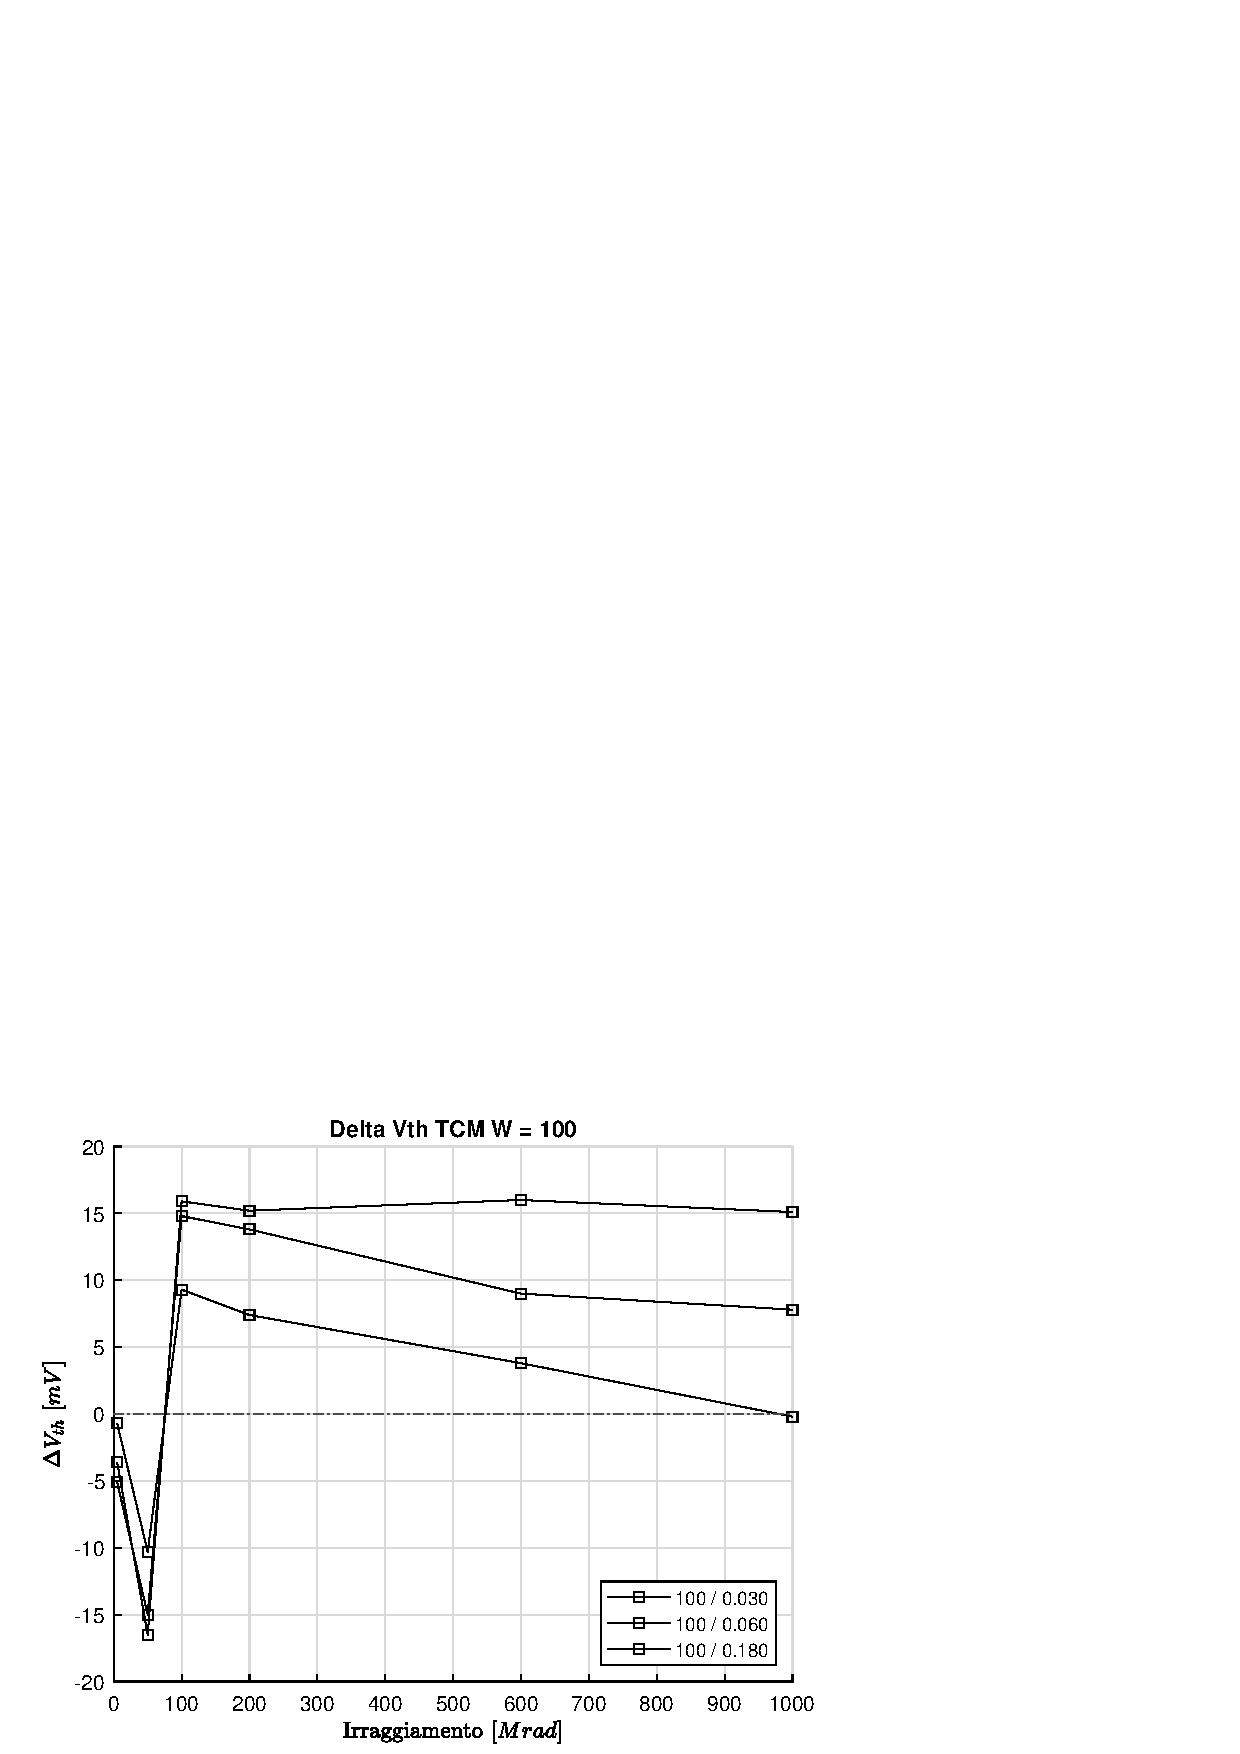
\includegraphics[width=0.49\textwidth]{./capitolo2/VTH/TCM/sovrapposizione-deltaVth-TCM-N100}
  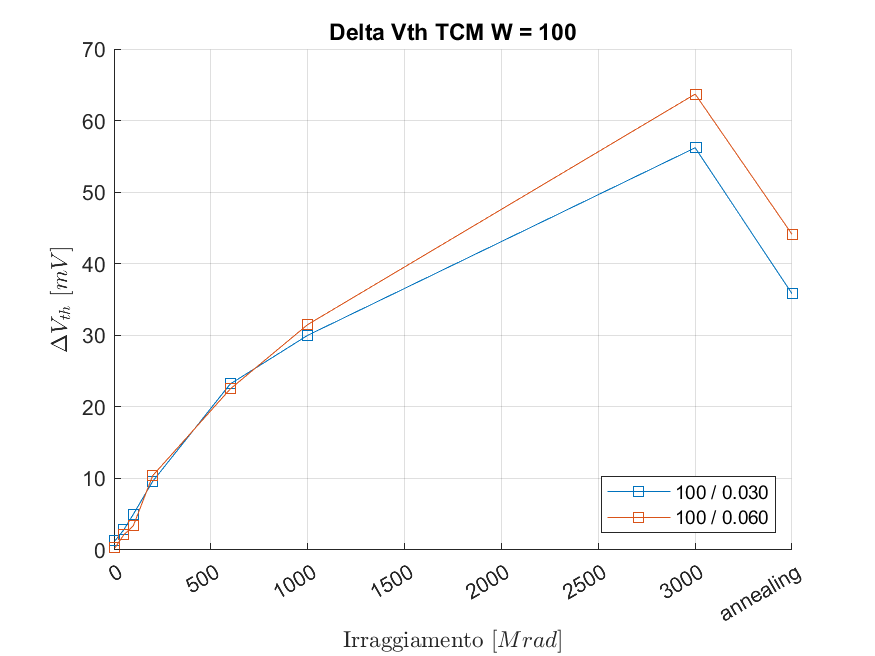
\includegraphics[width=0.49\textwidth]{./capitolo2/VTH/TCM/sovrapposizione-deltaVth-TCM-P100}
  %W = 200
  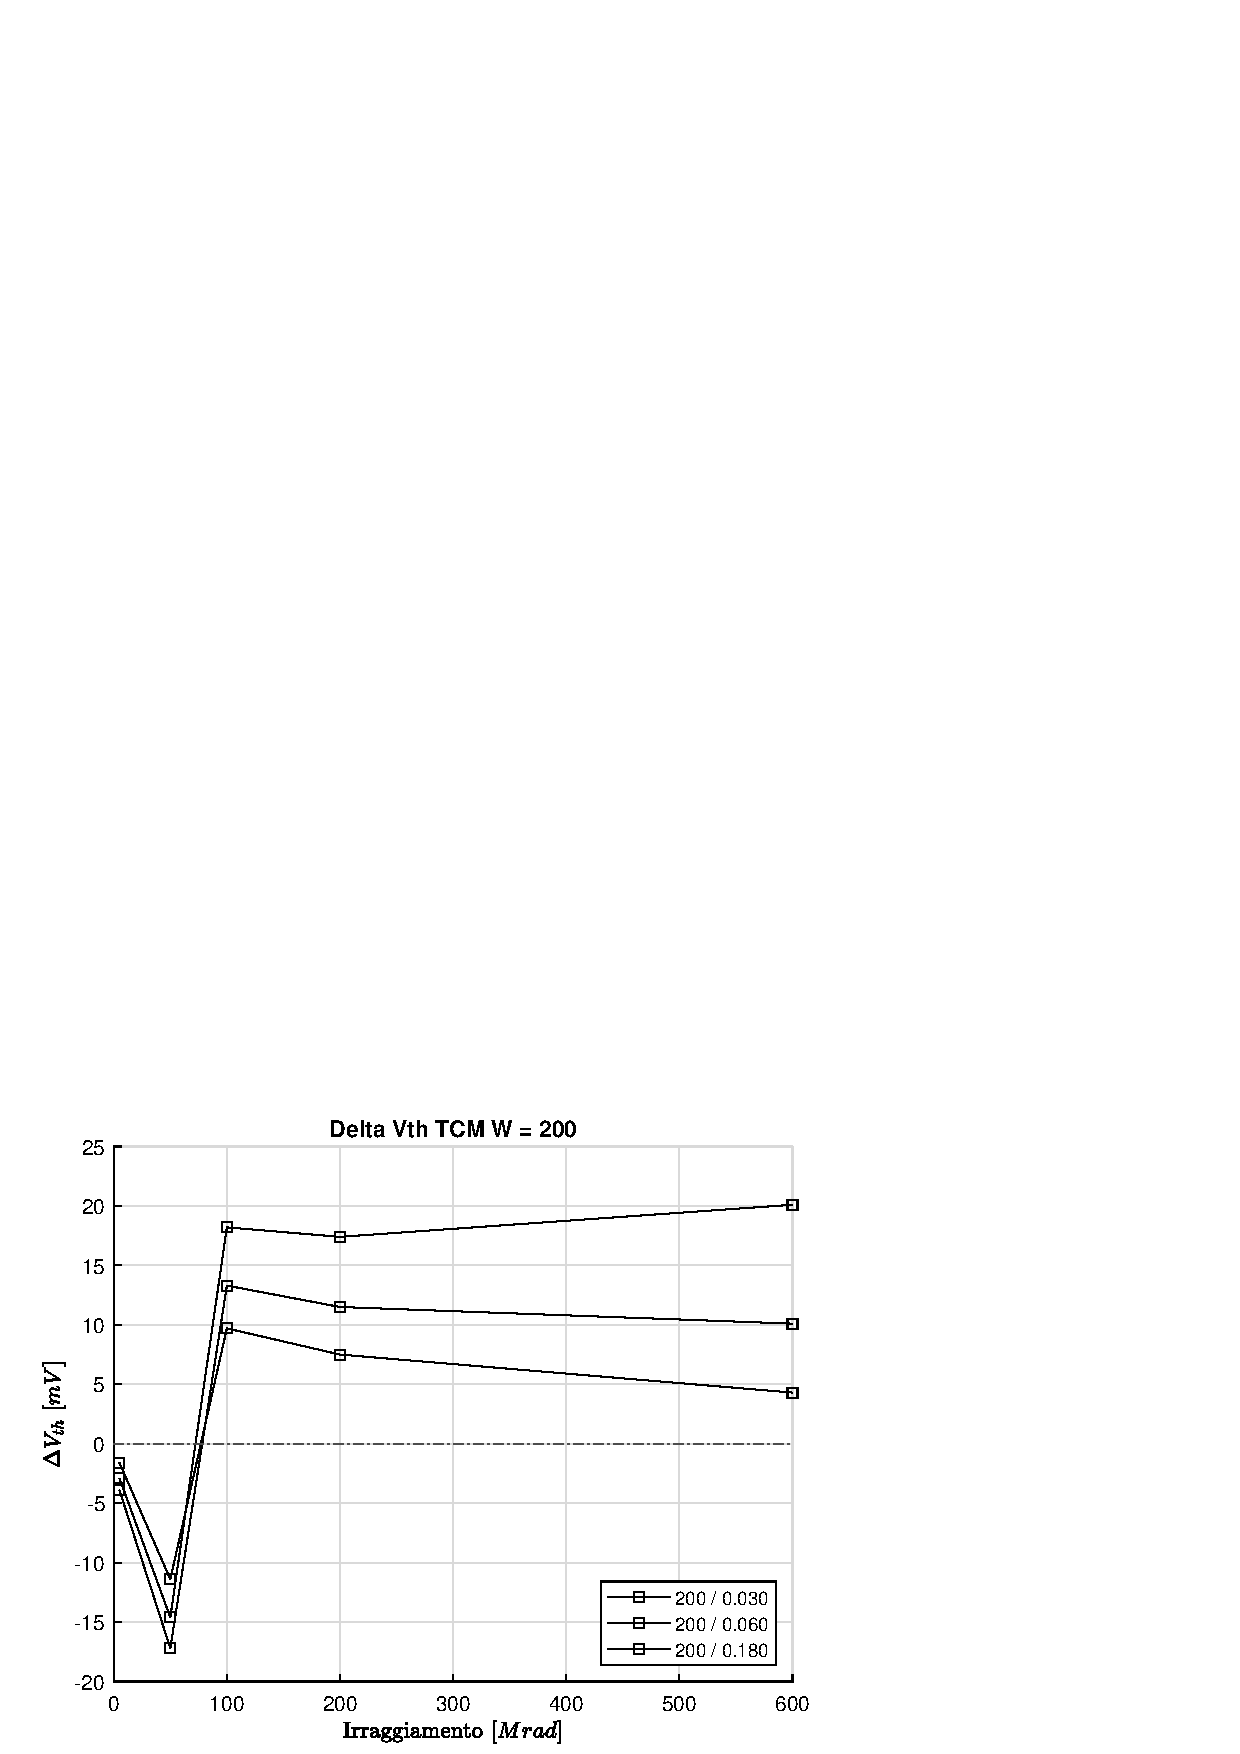
\includegraphics[width=0.49\textwidth]{./capitolo2/VTH/TCM/sovrapposizione-deltaVth-TCM-N200}
  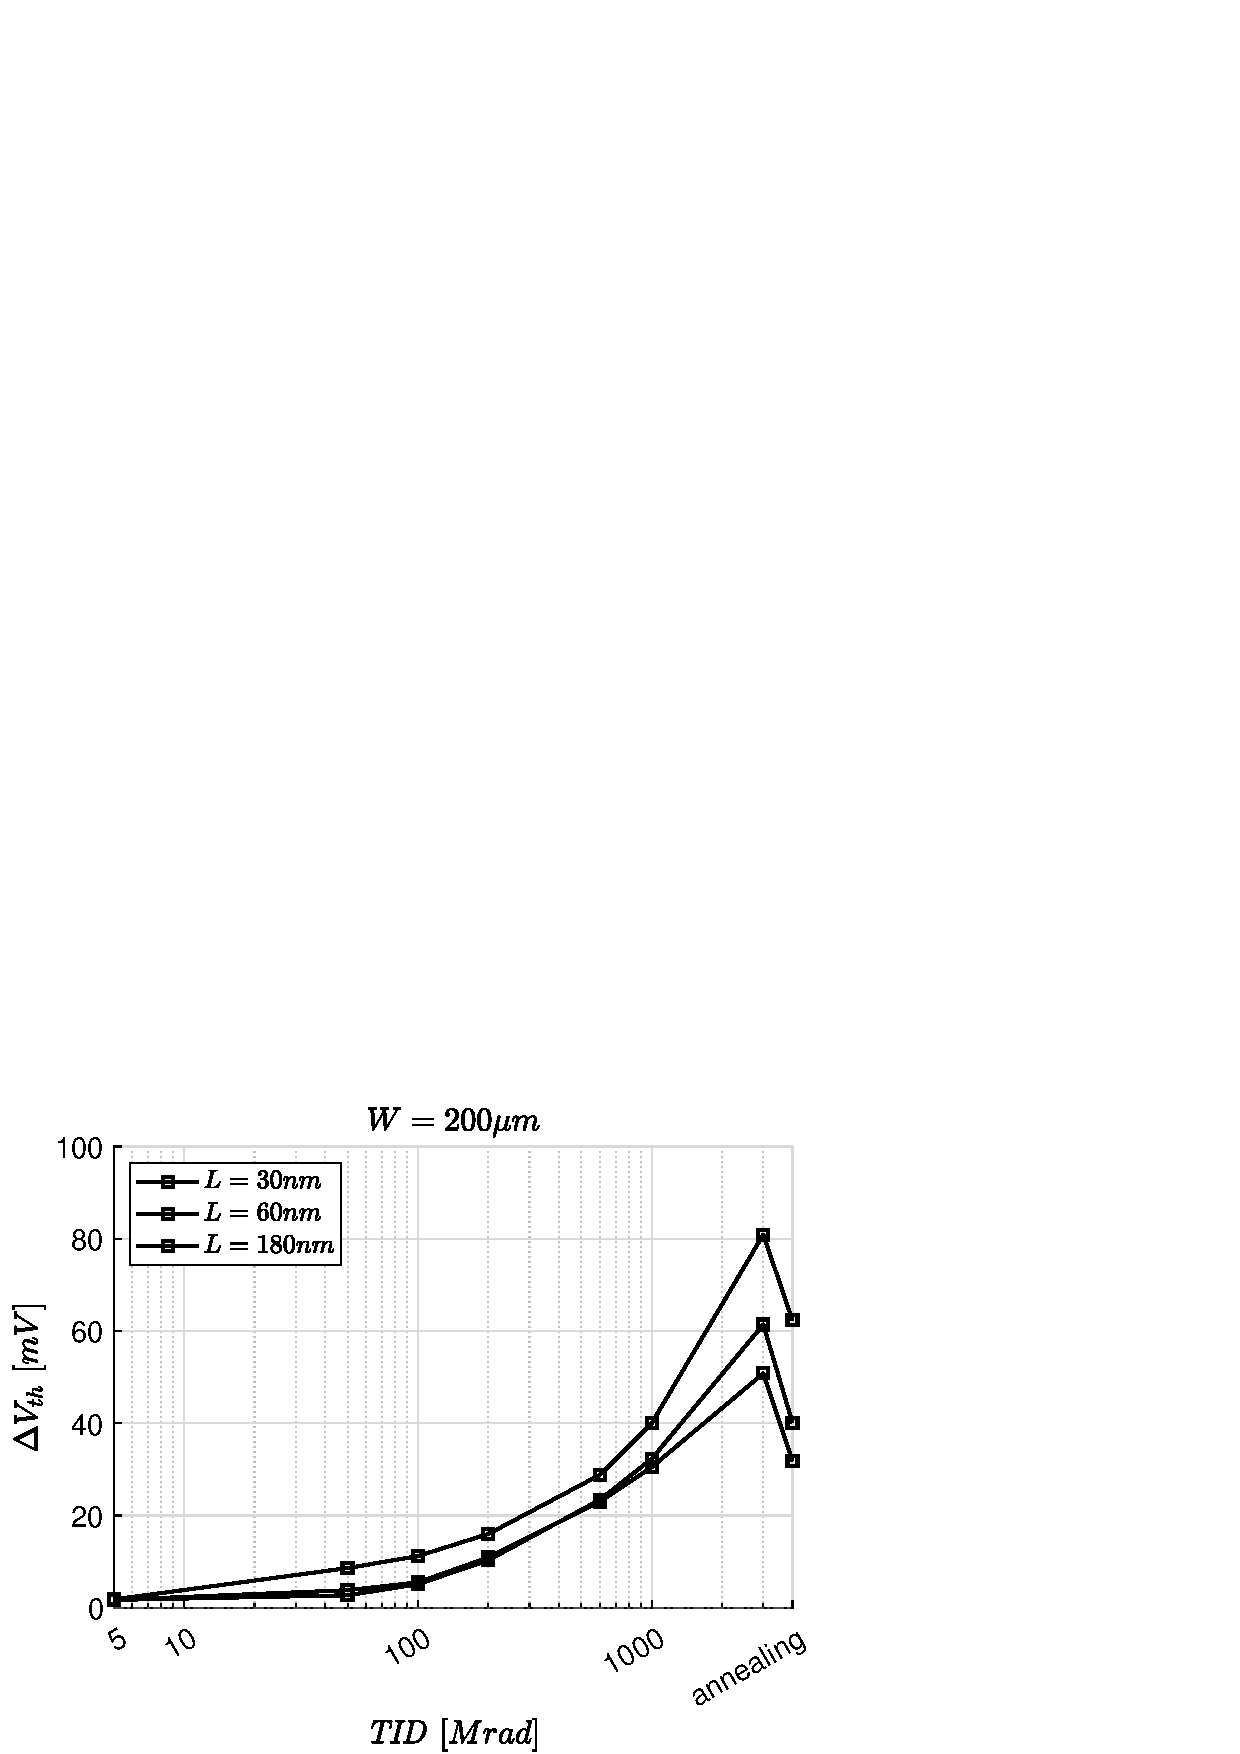
\includegraphics[width=0.49\textwidth]{./capitolo2/VTH/TCM/sovrapposizione-deltaVth-TCM-P200}
  %W = 600
  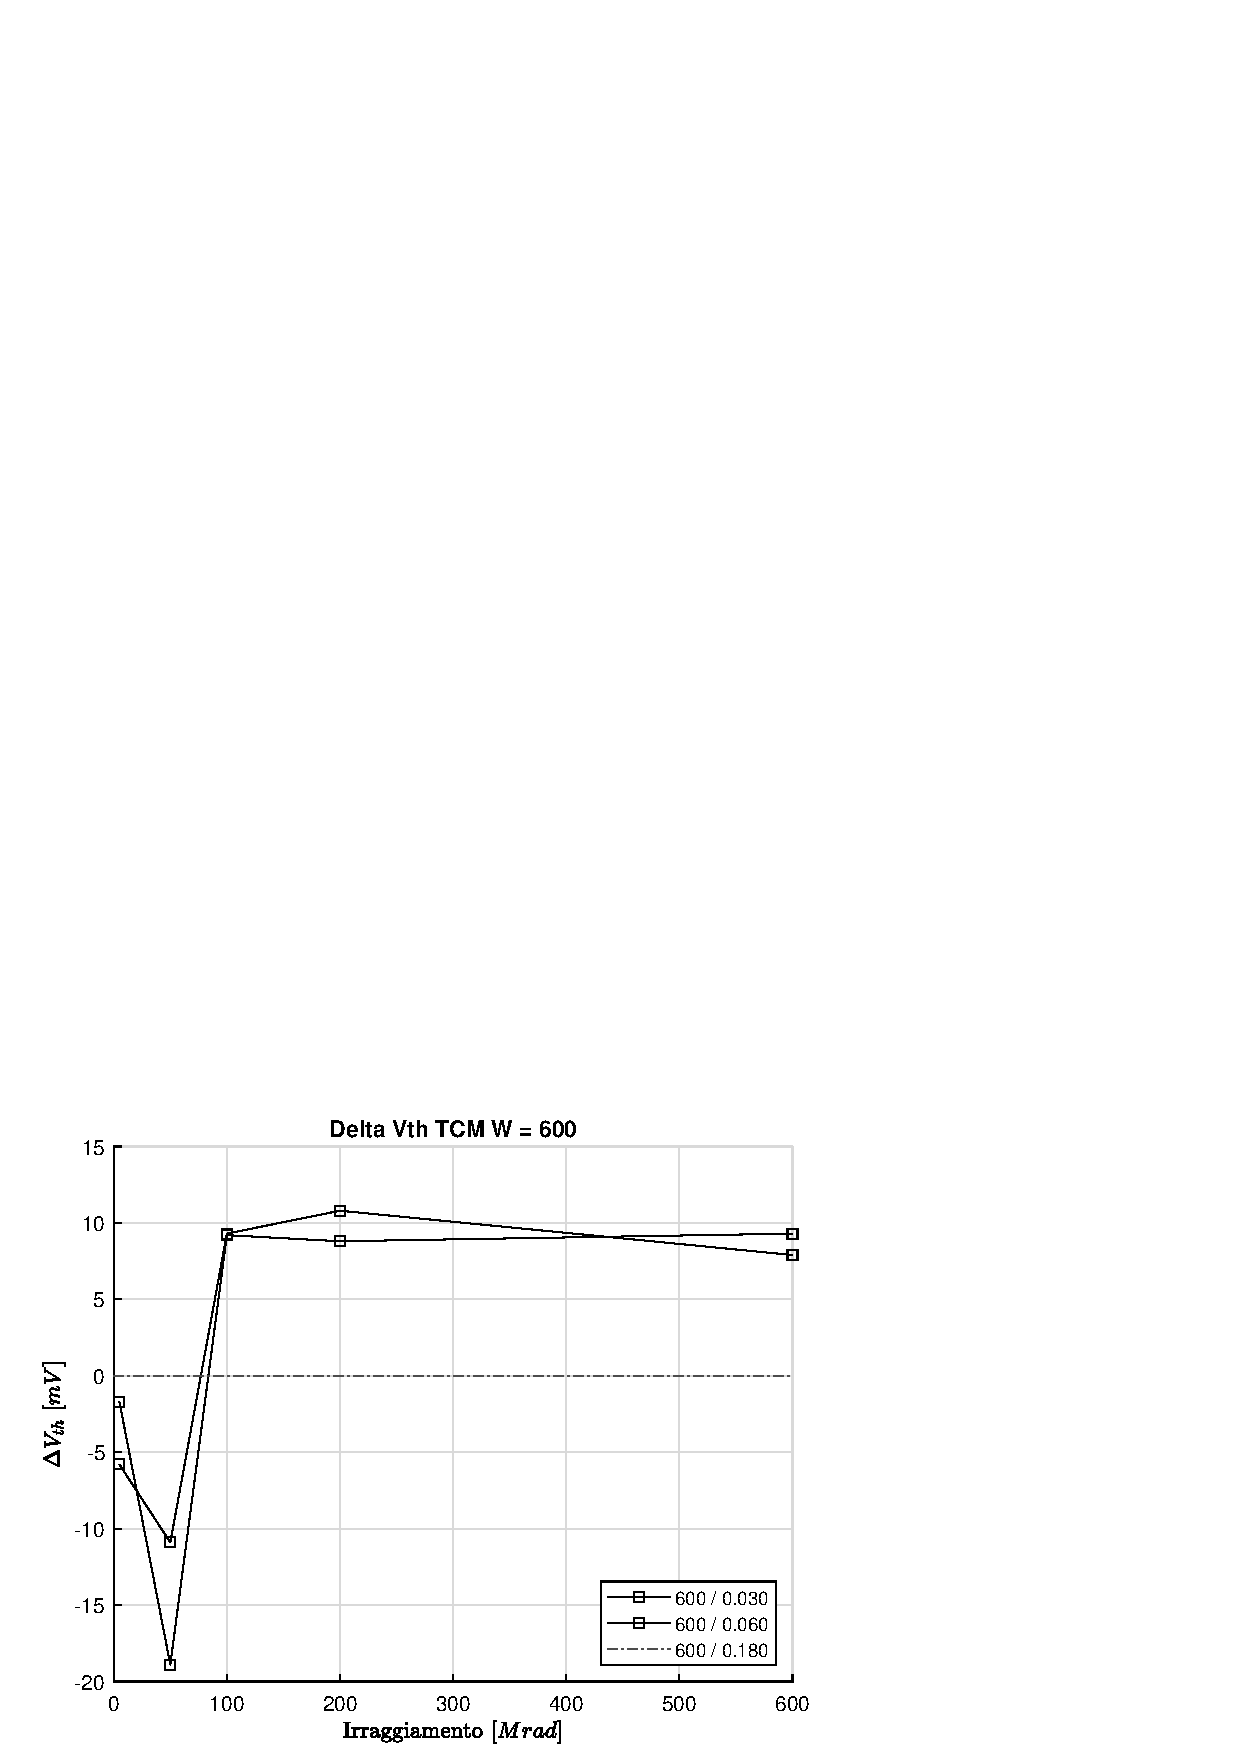
\includegraphics[width=0.49\textwidth]{./capitolo2/VTH/TCM/sovrapposizione-deltaVth-TCM-N600}
  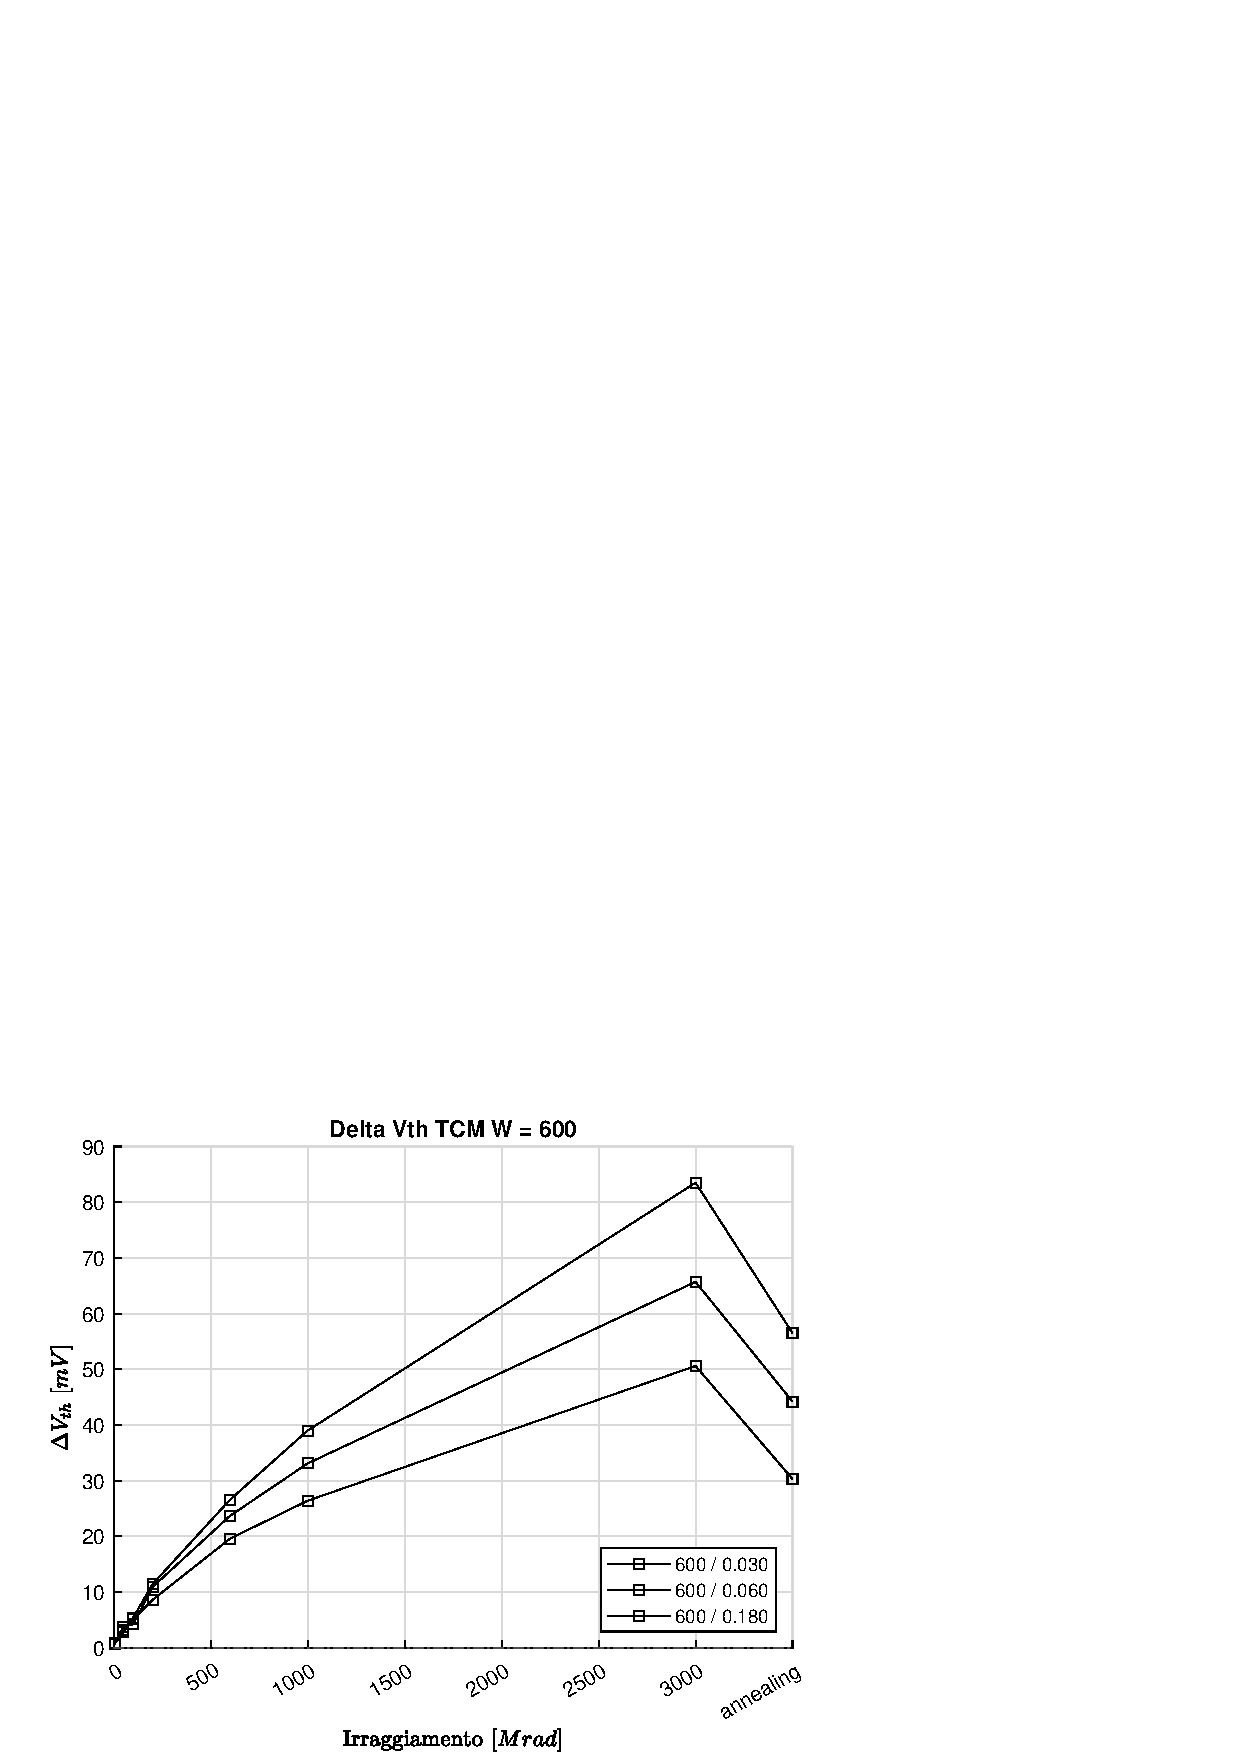
\includegraphics[width=0.49\textwidth]{./capitolo2/VTH/TCM/sovrapposizione-deltaVth-TCM-P600}

  \caption[Dati $\Delta V_{th}$ estratti con TCM]{Variazioni di $V_{th}$ dei dispositivi NMOS (a sinistra) e PMOS (a destra) estratte con \emph{TCM} in funzione della dose assorbita. Ogni figura si riferisce a una larghezza di canale W differente. Raggruppate per dimensione dello spessore dei dispositivi}
  \label{fig:deltaVthTCM}
\end{figure}

\subsection[SDLM]{Second Difference of the Logarithm of the drain current Minimum method}
Il secondo metodo analizzato è il \emph{Second Difference of the Logarithm of the drain current Minimum method, SDLM}. Questo metodo definisce la $V_{th}$ come la tensione $V_{GS}$ per la quale si ha il picco minimo della derivata seconda del logaritmo naturale di $I_D$ rispetto alla tensione di gate ($\frac{d^2lnI_D}{dV_{GS}^2}$) e vale solo per alti valori di $V_{DS}$\cite{art1}.


\begin{figure}[H]
  \centering
  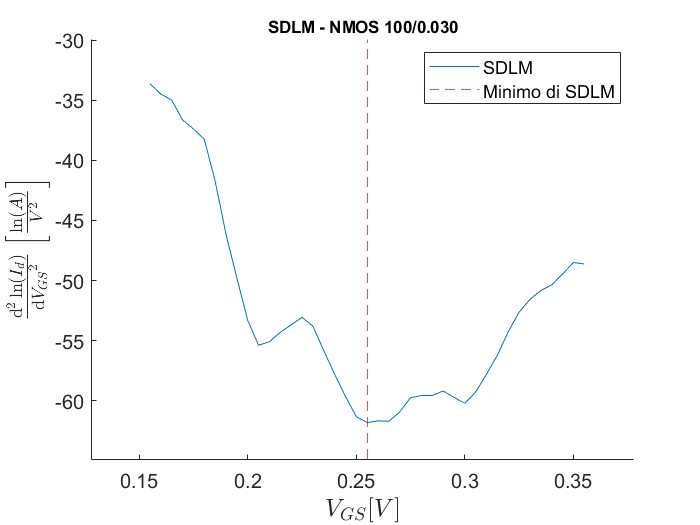
\includegraphics[width=0.49\textwidth]{./capitolo2/VTH/SDLM/SDLM-N4-100-30-NoFit}
  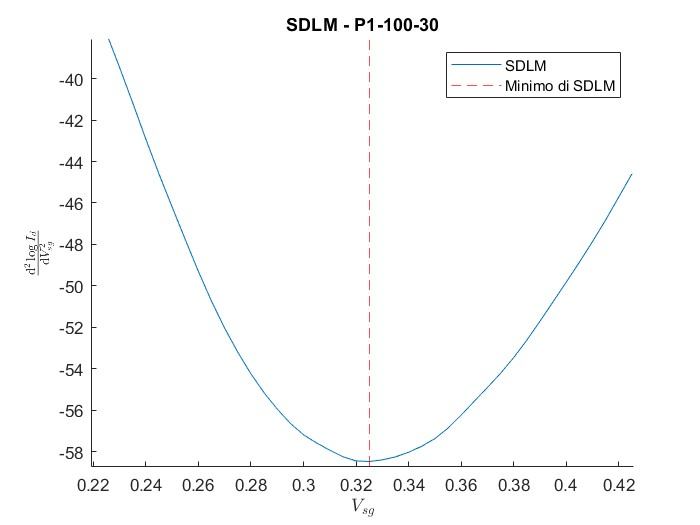
\includegraphics[width=0.49\textwidth]{./capitolo2/VTH/SDLM/SDLM-P1-100-30-NoFit}
  \caption[Applicazione SDLM senza fit polinomiale]{Esempio di \emph{SDLM} usato su un dispositivo NMOS e un dispositivo PMOS di dimensioni 100-0.030 a $V_{DS} = 900 mV$}
\end{figure}

Anche per questo metodo si ritrovano le problematiche presenti per il \emph{TCM}: si deve fare il fit di una curva ottenuta come derivata seconda e inoltre la risoluzione della $V_{GS}$ è $5mV$.
Quindi, anche per questo metodo, abbiamo deciso d'interpolare la funzione ottenuta con una polinomiale e considerare il minimo di quest'ultima.

% Tabella con i diversi gradi per SDLM
\begin{table}[h]
  \renewcommand{\arraystretch}{1.3}
  \centering
  \begin{tabular}{m{2.1cm} m{2cm} m{2cm} m{2cm} m{2cm}}
    \toprule
    \multirow{2}{*}{Dispositivo} & \multicolumn{4}{c}{$|V_{th}| [mV] \text{ con interpolante di grado:}$}                         \\
    \cmidrule{2-5}
                                 & 2                                                                    & 4     & 6     & 8     \\
    \midrule
    100 - 0.030                  & 332.0                                                                & 322.3 & 323.5 & 327.2 \\
    \hline
    100 - 0.060                  & 423.1                                                                & 416.1 & 411.6 & 411.7 \\
    \hline
    200 - 0.030                  & 303.2                                                                & 298.8 & 296.5 & 296.7 \\
    \hline
    200 - 0.060                  & 413.1                                                                & 404.4 & 404.9 & 405.0 \\
    \hline
    200 - 0.180                  & 460.4                                                                & 453.5 & 449.3 & 448.7 \\
    \hline
    600 - 0.030                  & 296.0                                                                & 291.4 & 289.7 & 298.1 \\
    \hline
    600 - 0.060                  & 398.3                                                                & 393.3 & 391.8 & 389.6 \\
    \hline
    600 - 0.180                  & 454.7                                                                & 446.7 & 441.4 & 441.3 \\
    \hline
  \end{tabular}
  \caption[Confronto $|V_{th}|$ al variare del grado del fit polinomiale con il metodo SDLM]{Confronto dei valori di $|V_{th}|$ dei dispositivi PMOS ottenuti con \emph{SDLM} con fit polinomiale di diversi gradi}
  \label{tab:GradiSDLM}
\end{table}

\begin{figure}[h!]
  \centering
  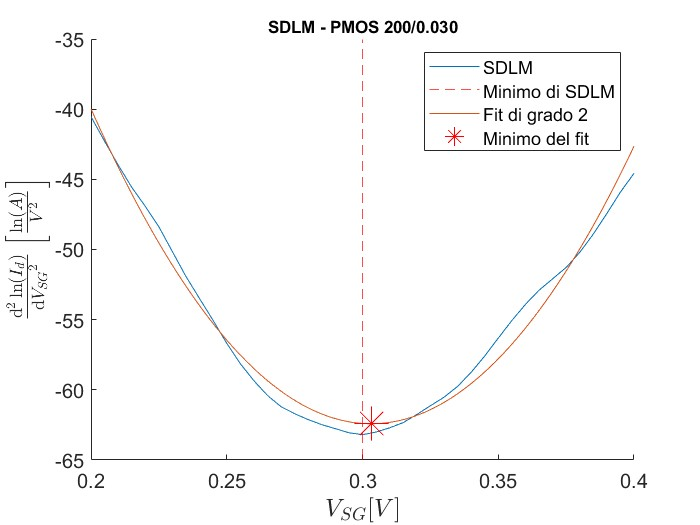
\includegraphics[width=0.49\textwidth]{./capitolo2/VTH/SDLM/SDLM-P1-200-30-grado2}
  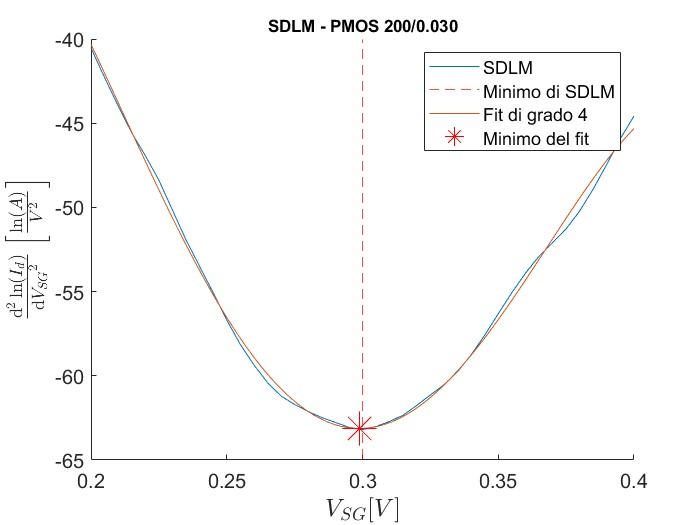
\includegraphics[width=0.49\textwidth]{./capitolo2/VTH/SDLM/SDLM-P1-200-30-grado4}
  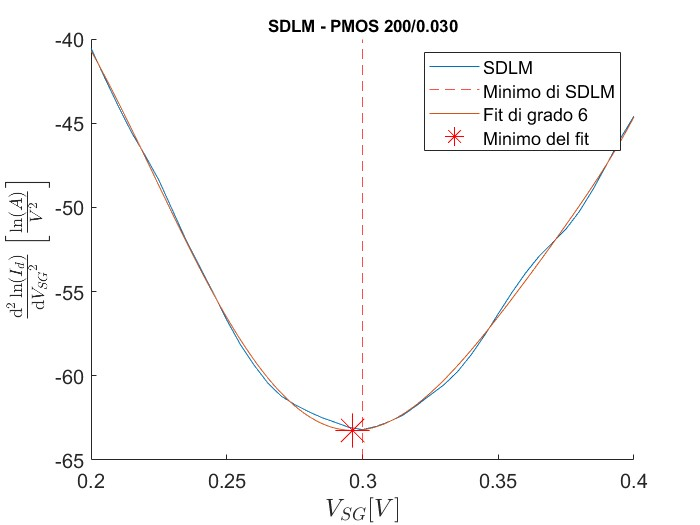
\includegraphics[width=0.49\textwidth]{./capitolo2/VTH/SDLM/SDLM-P1-200-30-grado6}
  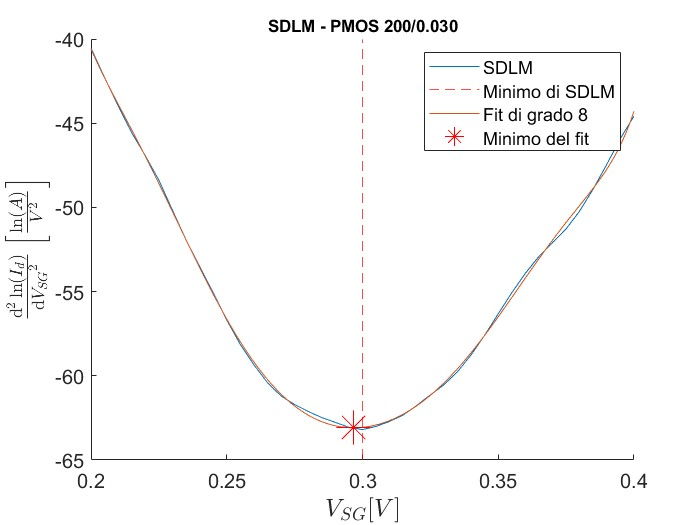
\includegraphics[width=0.49\textwidth]{./capitolo2/VTH/SDLM/SDLM-P1-200-30-grado8}
  \caption[Confronto SDLM tra diversi fit polinomiali a diversi gradi]{Confronto fra differenti fit (al variare del grado della funzione) della curva $\frac{d^2 \ln(I_D)}{d {V_{GS}}^2}$ per un dispositivo PMOS 200-0.030.}
  \label{fig:GradiSDLM}
\end{figure}

Prendendo in considerazione i dati presenti nella tabella \ref{tab:GradiSDLM}, si nota come $V_{th}$ assume valori molto diversi a seconda del grado della polinomiale interpolante. Nella maggior parte dei casi, le tensioni di soglia ottenute con polinomiali di grado basso (2 e 4) cambiano molto tra loro e rispetto a quelle ottenute con polinomiali di grado alto (6 e 8), mentre le misure ottenute con queste ultime sono, in genere, molto simili tra loro. Ad esempio, osservando i grafici relativi alla \emph{SDLM} del PMOS 200-0.030 (figura \ref{fig:GradiSDLM}), si può nota che il plot della funzione $\frac{d^2 \ln I_D}{dV_{GS}^2}$ ha un andamento che non viene interpolato in modo preciso da polinomiali di basso grado: per questo i valori minimi si discostano parecchio dai minimi ottenuti con polinomiali di grado maggiore. Risulta pertanto necessario estrarre le tensioni di soglia utilizzando una funzione polinomiale di grado 6.

Di seguito si riportano i valori delle $V_{th}$ e delle $\Delta V_{th}$, per i dispositivi NMOS: tabelle \ref{tab:VthSDLMN} e \ref{tab:deltaVthSDLMN}, e per i PMOS\footnote{Per i PMOS viene indicato il modulo della $V_{th}$ e per il calcolo della variazione si utilizza: $\Delta V_{th} = |V_{th_{post}}| - |V_{th_{pre}}|$.}: tabelle \ref{tab:VthSDLMP} e \ref{tab:deltaVthSDLMP}. Mentre in figura \ref{fig:deltaVthSDLM} si riportano i grafici che mostrano l'andamento della variazione della tensione di soglia ($\Delta V_{th}$), in funzione della dose assorbita.

\begin{table}[H]
  \renewcommand{\arraystretch}{1.3}
  \resizebox{\textwidth}{!}{%
    \begin{tabular}{c c c c c c c c c c }
      \toprule
      \multirow{2}{*}{Dispositivo} & \multicolumn{9}{c}{$V_{th} [mV] $}                                                                                          \\
      \cmidrule{2-10}
                                   & pre                                & $5Mrad$ & $50Mrad$ & $100Mrad$ & $200Mrad$ & $600Mrad$ & $1Grad$ & $3Grad$ & annealing \\
      \midrule
      100 - 0.030                  & 287.7                              & 259.5   & 271.2    & 289.8     & 287.7     & 278.5     & 276.4   & 269.7   & 275.0     \\
      \hline
      100 - 0.060                  & 356.8                              & 327.2   & 322.7    & 360.9     & 356.8     & 356.6     & 352.6   & 354.6   & 352.4     \\
      \hline
      100 - 0.180                  & 404.8                              & 381.5   & 369.1    & 422.1     & 404.8     & 422.1     & 418.2   & 433.1   & 442.5     \\
      \hline
      200 - 0.030                  & 279.7                              & 262.2   & 269.6    & 277.9     & 279.7     & 267.3     & 268.5   & 267.8   & 268.2     \\
      \hline
      200 - 0.060                  & 355.3                              & 325.4   & 313.3    & 357.4     & 355.3     & 351.1     & 348.7   & 355.7   & 358.2     \\
      \hline
      200 - 0.180                  & 417.9                              & 378.9   & 372.5    & 418.8     & 417.9     & 420.1     & 416.7   & 436.6   & 441.5     \\
      \hline
      600 - 0.060                  & 334.4                              & 276.0   & 304.0    & 336.1     & 334.4     & 332.7     & 331.6   & 333.8   & 336.7     \\
      \hline
      600 - 0.180                  & 417.1                              & 381.5   & 379.6    & 418.4     & 417.1     & 416.2     & 414.3   & 426.7   & 431.1     \\
      \bottomrule
    \end{tabular}%
  }
  \caption[$V_{th}$ dei dispositivi NMOS estratte con SDLM]{$V_{th}$ dei dispositivi NMOS estratte con \emph{SDLM}}
  \label{tab:VthSDLMN}
\end{table}

\begin{table}[H]
  \renewcommand{\arraystretch}{1.3}
  \resizebox{\textwidth}{!}{%
    \begin{tabular}{c c c c c c c c c c }
      \toprule
      \multirow{2}{*}{Dispositivo} & \multicolumn{9}{c}{$|V_{th}| [mV] $}                                                                                          \\
      \cmidrule{2-10}
                                   & pre                                & $5Mrad$ & $50Mrad$ & $100Mrad$ & $200Mrad$ & $600Mrad$ & $1Grad$ & $3Grad$ & annealing \\
      \midrule
      100 - 0.030                  & 323.5                              & 329.9   & 327.3    & 330.7     & 329.7     & 343.2     & 355.8   & 373.1   & 354.5     \\
      \hline
      100 - 0.060                  & 411.6                              & 409.9   & 412.3    & 415.5     & 416.8     & 428.3     & 435.8   & 466.9   & 453.9     \\
      \hline
      200 - 0.030                  & 296.5                              & 292.4   & 301.7    & 299.8     & 304.4     & 320.0     & 323.0   & 345.6   & 327.0     \\
      \hline
      200 - 0.060                  & 404.9                              & 403.9   & 405.3    & 407.3     & 413.0     & 422.5     & 430.9   & 460.0   & 442.1     \\
      \hline
      200 - 0.180                  & 449.3                              & 452.1   & 457.6    & 456.9     & 461.9     & 473.7     & 482.7   & 520.4   & 506.6     \\
      \hline
      600 - 0.030                  & 289.7                              & 293.0   & 297.3    & 297.0     & 299.9     & 313.1     & 325.7   & 345.2   & 324.0     \\
      \hline
      600 - 0.060                  & 391.8                              & 393.4   & 397.4    & 396.8     & 402.0     & 415.1     & 421.2   & 451.1   & 432.6     \\
      \hline
      600 - 0.180                  & 441.4                              & 443.4   & 445.1    & 444.6     & 450.9     & 464.5     & 474.2   & 514.2   & 492.4     \\
      \bottomrule
    \end{tabular}%
  }
  \caption[$|V_{th}|$ dei dispositivi PMOS estratte con SDLM]{$|V_{th}|$ dei dispositivi PMOS estratte con \emph{SDLM}}
  \label{tab:VthSDLMP}
\end{table}


\begin{table}[H]
  \renewcommand{\arraystretch}{1.3}
  \resizebox{\textwidth}{!}{%
    \begin{tabular}{c c c c c c c c c}
      \toprule
      \multirow{2}{*}{Dispositivo} & \multicolumn{8}{c}{$\Delta V_{th} [mV] $}                                                                                \\
      \cmidrule{2-9}
                                   & $5Mrad$                                   & $50Mrad$ & $100Mrad$ & $200Mrad$ & $600Mrad$ & $1Grad$ & $3Grad$ & annealing \\
      \midrule
      100 - 0.030                  & -20.2                                     & -8.5     & 10.1      & 8.0       & -1.2      & -3.3    & -10.0   & -4.7      \\
      \hline
      100 - 0.060                  & 12.1                                      & 7.6      & 45.8      & 41.7      & 41.5      & 37.5    & 39.5    & 37.3      \\
      \hline
      100 - 0.180                  & 12.1                                      & -0.3     & 52.7      & 35.4      & 52.7      & 48.8    & 63.7    & 73.1      \\
      \hline
      200 - 0.030                  & -2.5                                      & 4.9      & 13.2      & 15.0      & 2.6       & 3.8     & 3.1     & 3.5       \\
      \hline
      200 - 0.060                  & -0.6                                      & -12.7    & 31.4      & 29.3      & 25.1      & 22.7    & 29.7    & 32.2      \\
      \hline
      200 - 0.180                  & 7.1                                       & 0.7      & 47.0      & 46.1      & 48.3      & 44.9    & 64.8    & 69.7      \\
      \hline
      600 - 0.060                  & -29.1                                     & -1.1     & 31.0      & 29.3      & 27.6      & 26.5    & 28.7    & 31.6      \\
      \hline
      600 - 0.180                  & -3.3                                      & --5.2    & 33.6      & 32.3      & 31.4      & 29.5    & 41.9    & 46.3      \\
      \bottomrule
    \end{tabular}%
  }
  \caption[$\Delta V_{th}$ dei dispositivi NMOS estratte con SDLM]{$\Delta V_{th}$ dei dispositivi NMOS estratte con \emph{SDLM}}
  \label{tab:deltaVthSDLMN}
\end{table}

\begin{table}[H]
  \renewcommand{\arraystretch}{1.3}
  \resizebox{\textwidth}{!}{%
    \begin{tabular}{c c c c c c c c c}
      \toprule
      \multirow{2}{*}{Dispositivo} & \multicolumn{8}{c}{$\Delta V_{th} [mV] $}                                                                                \\
      \cmidrule{2-9}
                                   & $5Mrad$                                   & $50Mrad$ & $100Mrad$ & $200Mrad$ & $600Mrad$ & $1Grad$ & $3Grad$ & annealing \\
      \midrule
      100 - 0.030                  & 6.4                                       & 3.8      & 7.2       & 6.2       & 19.7      & 32.3    & 49.6    & 31.0      \\
      \hline
      100 - 0.060                  & -1.7                                      & 0.7      & 3.9       & 5.2       & 16.7      & 24.2    & 55.3    & 42.3      \\
      \hline
      200 - 0.030                  & -4.1                                      & 5.2      & 3.3       & 7.9       & 23.5      & 26.5    & 49.1    & 30.5      \\
      \hline
      200 - 0.060                  & -1.0                                      & 0.4      & 2.4       & 8.1       & 17.6      & 26.0    & 55.1    & 37.2      \\
      \hline
      200 - 0.180                  & 2.8                                       & 8.3      & 7.6       & 12.6      & 24.4      & 33.4    & 71.1    & 57.3      \\
      \hline
      600 - 0.030                  & 3.3                                       & 7.6      & 7.3       & 10.2      & 23.4      & 36.0    & 55.5    & 34.3      \\
      \hline
      600 - 0.060                  & 1.6                                       & 5.6      & 5.0       & 10.2      & 23.3      & 29.4    & 59.3    & 40.8      \\
      \hline
      600 - 0.180                  & 2.0                                       & 3.7      & 3.2       & 9.5       & 23.1      & 32.8    & 72.8    & 51.0      \\
      \bottomrule
    \end{tabular}%
  }
  \caption[$\Delta V_{th}$ dei dispositivi PMOS estratte con SDLM]{$\Delta V_{th}$ dei dispositivi PMOS estratte con \emph{SDLM}}
  \label{tab:deltaVthSDLMP}
\end{table}

% Plot Delta Vth, SDLM
\begin{figure}[H]
  \centering
  %W = 100
  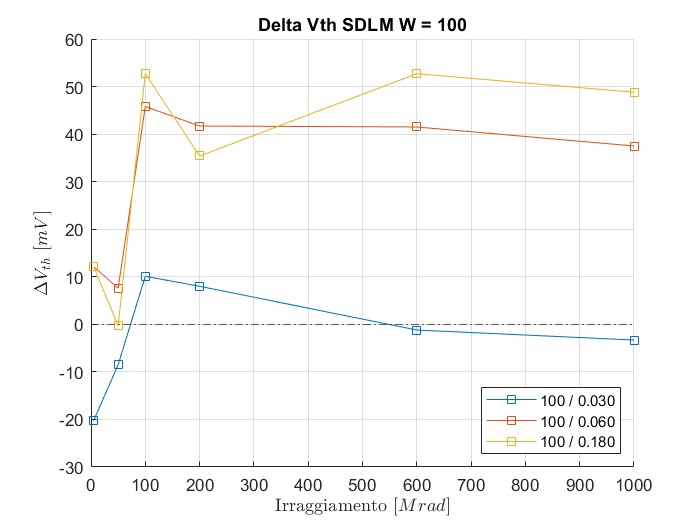
\includegraphics[width=0.49\textwidth]{./capitolo2/VTH/SDLM/sovrapposizione-deltaVth-SDLM-N100}
  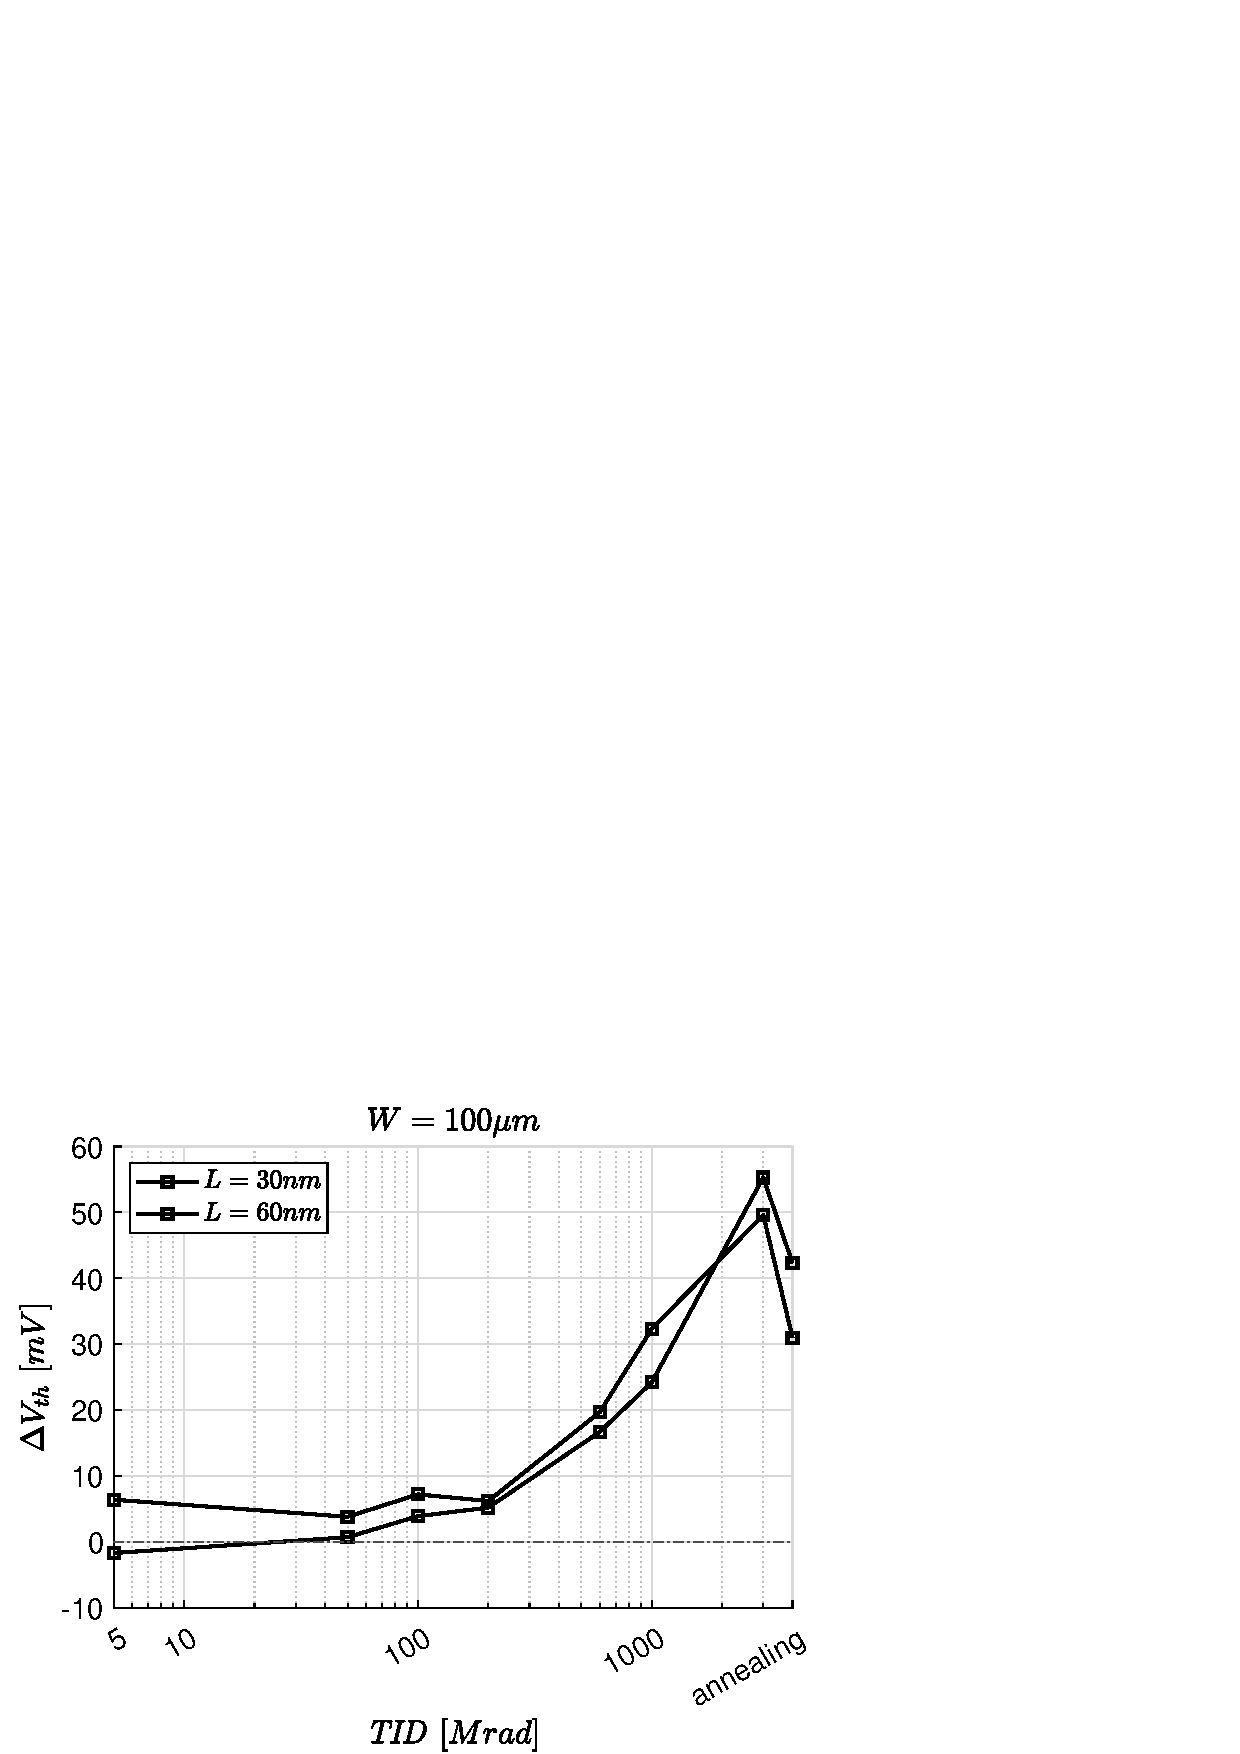
\includegraphics[width=0.49\textwidth]{./capitolo2/VTH/SDLM/sovrapposizione-deltaVth-SDLM-P100}
  %W = 200
  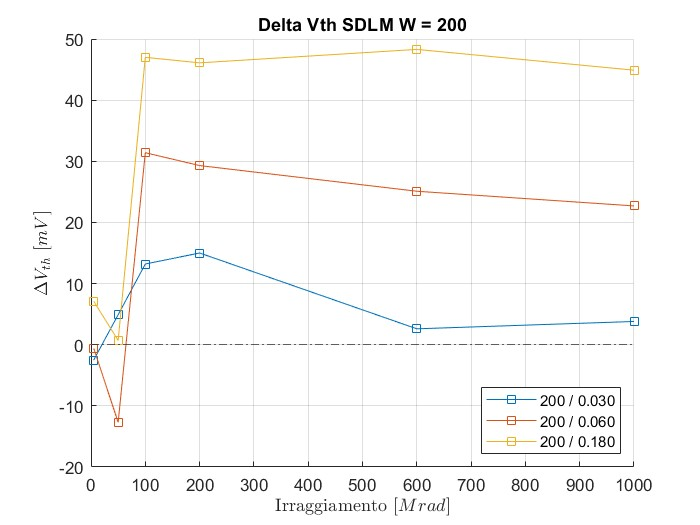
\includegraphics[width=0.49\textwidth]{./capitolo2/VTH/SDLM/sovrapposizione-deltaVth-SDLM-N200}
  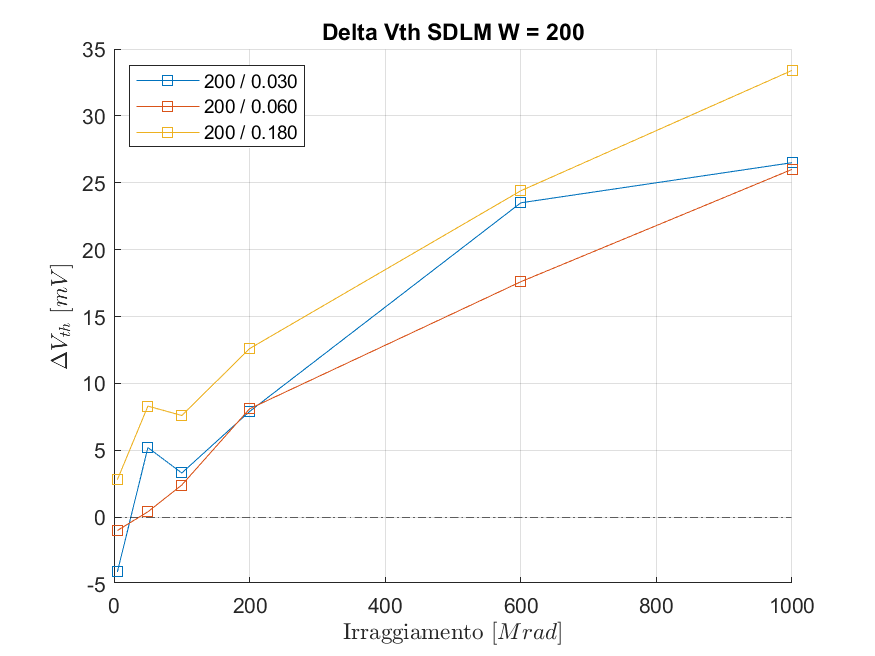
\includegraphics[width=0.49\textwidth]{./capitolo2/VTH/SDLM/sovrapposizione-deltaVth-SDLM-P200}
  %W = 600
  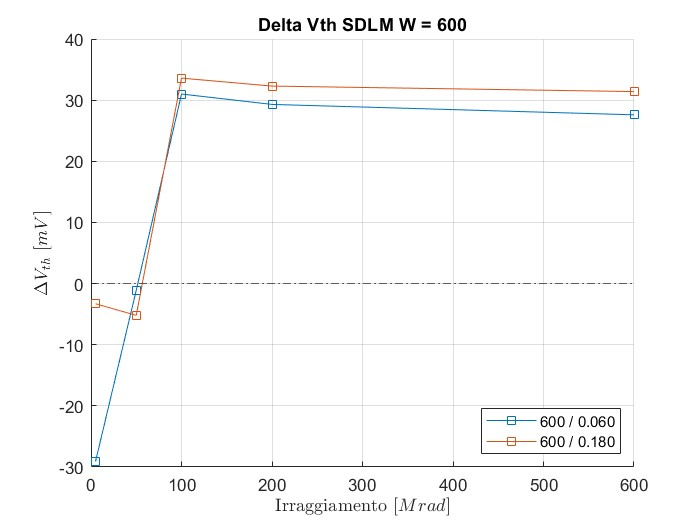
\includegraphics[width=0.49\textwidth]{./capitolo2/VTH/SDLM/sovrapposizione-deltaVth-SDLM-N600}
  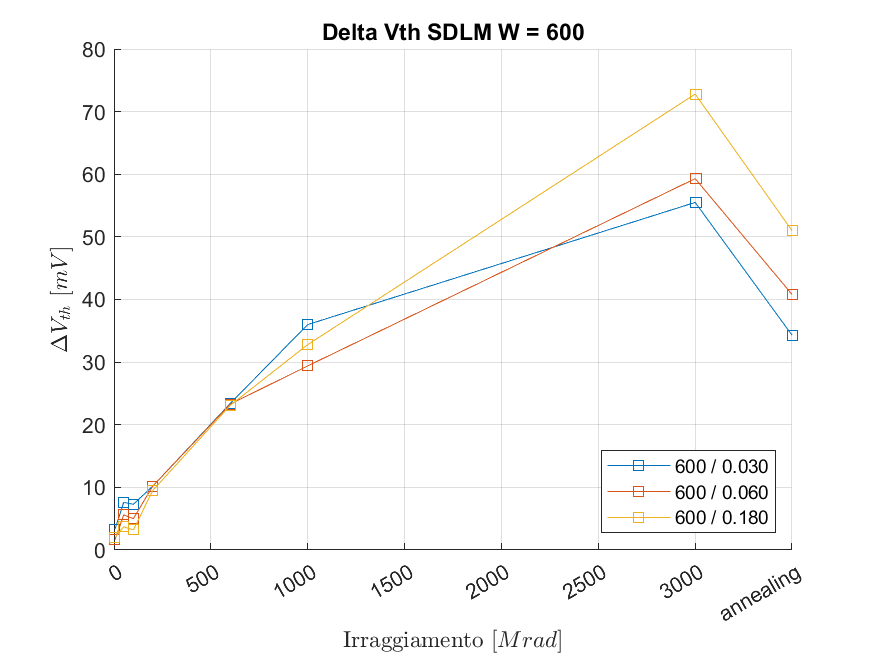
\includegraphics[width=0.49\textwidth]{./capitolo2/VTH/SDLM/sovrapposizione-deltaVth-SDLM-P600}
  \caption[Dati $\Delta V_{th}$ estratti con SDLM]{Variazioni di $V_{th}$ dei dispositivi NMOS (a sinistra) PMOS (a destra) estratte con \emph{SDLM} in funzione della dose assorbita. Ogni figura si riferisce a una larghezza di canale W differente. Raggruppate per dimensione dello spessore dei dispositivi}
  \label{fig:deltaVthSDLM}
\end{figure}

\subsection[ELR]{Extrapolation in the Linear Region method}
Il terzo metodo analizzato è l'\emph{Extrapolation in the Linear Region method, ELR}\cite{art2}. La tensione di soglia estratta con questo metodo è data dall'intercetta della estrapolazione lineare della caratteristica $I_D-V_{GS}$ nel suo punto di massima pendenza (cioè il punto di massima transconduttanza, $g_m$) con l'asse delle ascisse ($V_{GS}$). Alla tensione così ottenuta, per ottenere la tensione di soglia, si dovrà aggiungere $V_{DS}/2$, dove $V_{DS}$ è la tensione alla quale è stata misurata la caratteristica $I_D-V_{GS}$ interpolata linearmente.
Operativamente, il tratto sul quale fare il fit lineare è ottenuto prendendo un determinato intervallo nell'intorno del punto di flesso della $I_D-V_{GS}$.

\begin{figure}[h!]
  \centering
  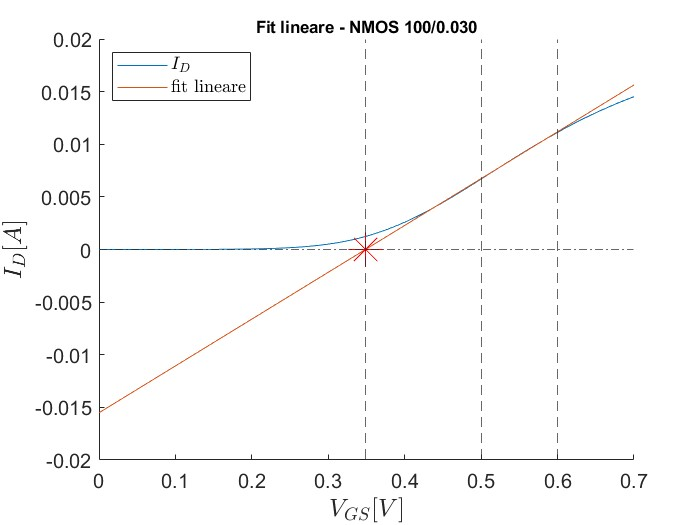
\includegraphics[width=0.49\textwidth]{./capitolo2/VTH/ELR/LinearFit-N4-100-30}
  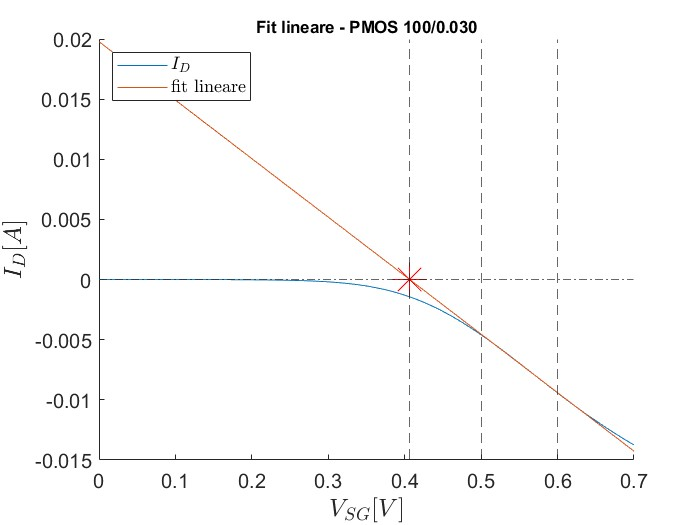
\includegraphics[width=0.49\textwidth]{./capitolo2/VTH/ELR/LinearFit-P1-100-30}
  \caption[Applicazione ELR]{Fit lineare della caratteristica  $I_D$-$V_{GS}$ a $V_{DS}=150mV$ di un NMOS e di un PMOS di dimensioni 100-0.030 }
\end{figure}

Lo svantaggio principale di questo metodo è dato dal fatto che il punto di pendenza massima può essere incerto a causa di possibili effetti quali il degrado della mobilità dei portatori di carica e la possibile presenza di resistenze parassite serie al terminale di source e drain.
Nonostante ciò, per il nostro studio questo metodo potrebbe risultare efficace, in quanto non siamo principalmente interessati al valore della tensione di soglia dei dispositivi, ma alla variazione della tensione di soglia a causa delle radiazioni ionizzanti alle quali i dispositivi vengono sottoposti. Dunque gli errori prodotti dalle resistenze parassite e dalla degradazione di mobilità possono essere considerate come un offset che viene eliminato nel momento in cui si calcola la differenza tra la $V_{th}$ pre e post irraggiamento.\\
È infine doveroso fare una parentesi sulla regione di linearizzazione considerata per questo studio: infatti non è possibile stabilire con certezza una regione fissa in cui la funzione, ottenuta con misure sperimentali, può essere linearizzata. Il metodo da noi applicato è stato quello di analizzare tutti i possibili intervalli di linearizzazione ampi $100 mV$ i cui estremi ricadono nell'intervallo $[300 mV ; 750mV]$ e scegliere quello il cui il fit approssimava meglio la funzione. All'atto pratico abbiamo considerato l'intervallo il cui fit ha il coefficiente di determinazione $R^2$ piu alto, che è risultato essere sempre maggiore di $0.999$.


\begin{table}[H]
  \renewcommand{\arraystretch}{1.3}
  \resizebox{\textwidth}{!}{%
    \begin{tabular}{c c c c c c c c c c }
      \toprule
      \multirow{2}{*}{Dispositivo} & \multicolumn{9}{c}{$V_{th} [mV] $}                                                                                          \\
      \cmidrule{2-10}
                                   & pre                                & $5Mrad$ & $50Mrad$ & $100Mrad$ & $200Mrad$ & $600Mrad$ & $1Grad$ & $3Grad$ & annealing \\
      \midrule
      100 - 0.030                  & 351.0                              & 348.5   & 338.8    & 360.4     & 358.4     & 353.1     & 348.6   & 346.2   & 350.1     \\
      \hline
      100 - 0.060                  & 388.8                              & 385.3   & 373.1    & 403.8     & 402.0     & 398.8     & 396.0   & 399.6   & 404.4     \\
      \hline
      100 - 0.180                  & 465.9                              & 461.6   & 449.4    & 482.5     & 481.7     & 482.3     & 481.9   & 492.9   & 500.8     \\
      \hline
      200 - 0.030                  & 336.9                              & 334.6   & 324.6    & 346.0     & 344.7     & 341.3     & 338.7   & 340.1   & 344.5     \\
      \hline
      200 - 0.060                  & 382.9                              & 379.4   & 366.4    & 396.6     & 395.1     & 393.4     & 391.6   & 397.6   & 403.1     \\
      \hline
      200 - 0.180                  & 454.6                              & 449.8   & 438.1    & 471.1     & 471.0     & 473.6     & 474.4   & 489.5   & 497.8     \\
      \hline
      600 - 0.060                  & 349.3                              & 347.2   & 336.7    & 361.2     & 361.4     & 358.1     & 356.7   & 359.9   & 366.0     \\
      \hline
      600 - 0.180                  & 431.8                              & 427.5   & 412.4    & 440.6     & 440.1     & 440.8     & 440.4   & 451.3   & 460.8     \\
      \bottomrule
    \end{tabular}%
  }
  \caption[$V_{th}$ dei dispositivi NMOS estratte con ELR]{$V_{th}$ dei dispositivi NMOS estratte con \emph{ELR}}
  \label{tab:VthELRN}
\end{table}

\begin{table}[H]
  \renewcommand{\arraystretch}{1.3}
  \resizebox{\textwidth}{!}{%
    \begin{tabular}{c c c c c c c c c c }
      \toprule
      \multirow{2}{*}{Dispositivo} & \multicolumn{9}{c}{$|V_{th}| [mV] $}                                                                                          \\
      \cmidrule{2-10}
                                   & pre                                & $5Mrad$ & $50Mrad$ & $100Mrad$ & $200Mrad$ & $600Mrad$ & $1Grad$ & $3Grad$ & annealing \\
      \midrule
      100 - 0.030                  & 405.8                              & 406.6   & 408.6    & 410.1     & 416.1     & 429.3     & 436.6   & 458.9   & 440.7     \\
      \hline
      100 - 0.060                  & 452.0                              & 452.9   & 454.6    & 456.5     & 462.9     & 475.4     & 484.9   & 515.9   & 497.1     \\
      \hline
      200 - 0.030                  & 376.2                              & 377.6   & 379.3    & 380.3     & 386.9     & 397.5     & 404.7   & 426.3   & 406.6     \\
      \hline
      200 - 0.060                  & 434.6                              & 435.9   & 437.5    & 439.3     & 445.1     & 458.1     & 467.2   & 495.9   & 474.2     \\
      \hline
      200 - 0.180                  & 482.3                              & 483.5   & 490.3    & 492.4     & 498.5     & 511.5     & 522.6   & 562.3   & 543.2     \\
      \hline
      600 - 0.030                  & 359.4                              & 360.9   & 362.5    & 364.6     & 370.1     & 379.8     & 387.1   & 410.6   & 389.2     \\
      \hline
      600 - 0.060                  & 412.8                              & 414.2   & 417.1    & 417.5     & 424.5     & 437.3     & 446.1   & 477.9   & 455.5     \\
      \hline
      600 - 0.180                  & 463.2                              & 464.4   & 466.4    & 468.9     & 475.2     & 490.8     & 502.9   & 546.2   & 519.3     \\
      \bottomrule
    \end{tabular}%
  }
  \caption[$|V_{th}|$ dei dispositivi PMOS estratte con ELR]{$|V_{th}|$ dei dispositivi PMOS estratte con \emph{ELR}}
  \label{tab:VthELRP}
\end{table}



\begin{table}[H]
  \renewcommand{\arraystretch}{1.3}
  \resizebox{\textwidth}{!}{%
    \begin{tabular}{c c c c c c c c c}
      \toprule
      \multirow{2}{*}{Dispositivo} & \multicolumn{8}{c}{$\Delta V_{th} [mV] $}                                                                                \\
      \cmidrule{2-9}
                                   & $5Mrad$                                   & $50Mrad$ & $100Mrad$ & $200Mrad$ & $600Mrad$ & $1Grad$ & $3Grad$ & annealing \\
      \midrule
      100 - 0.030                  & -2.5                                      & -12.1    & 9.4       & 7.4       & 2.1       & -2.4    & -4.8    & -0.9      \\
      \hline
      100 - 0.060                  & -3.5                                      & -15.8    & 15.0      & 13.1      & 10.0      & 7.2     & 10.8    & 15.6      \\
      \hline
      100 - 0.180                  & -4.3                                      & -16.5    & 16.6      & 15.8      & 16.3      & 16.0    & 27.0    & 34.9      \\
      \hline
      200 - 0.030                  & -2.3                                      & -12.3    & 9.1       & 7.9       & 4.5       & 1.8     & 3.2     & 7.6       \\
      \hline
      200 - 0.060                  & -3.5                                      & -16.5    & 13.6      & 12.2      & 10.5      & 8.7     & 14.7    & 20.2      \\
      \hline
      200 - 0.180                  & -4.9                                      & -16.5    & 16.5      & 16.4      & 19.1      & 19.8    & 34.9    & 43.2      \\
      \hline
      600 - 0.060                  & -2.2                                      & -12.7    & 11.8      & 12.0      & 8.8       & 7.4     & 10.6    & 16.7      \\
      \hline
      600 - 0.180                  & -4.3                                      & -19.4    & 8.8       & 8.2       & 9.0       & 8.6     & 19.5    & 29.0      \\
      \bottomrule
    \end{tabular}%
  }
  \caption[$\Delta V_{th}$ dei dispositivi NMOS estratte con ELR]{$\Delta V_{th}$ dei dispositivi NMOS estratte con \emph{ELR}}
  \label{tab:deltaVthELRN}
\end{table}


\begin{table}[H]
  \renewcommand{\arraystretch}{1.3}
  \resizebox{\textwidth}{!}{%
    \begin{tabular}{c c c c c c c c c}
      \toprule
      \multirow{2}{*}{Dispositivo} & \multicolumn{8}{c}{$\Delta V_{th} [mV] $}                                                                                \\
      \cmidrule{2-9}
                                   & $5Mrad$                                   & $50Mrad$ & $100Mrad$ & $200Mrad$ & $600Mrad$ & $1Grad$ & $3Grad$ & annealing \\
      \midrule

      100 - 0.030                  & 0.8                                       & 2.8      & 4.4       & 10.4      & 23.5      & 30.8    & 53.1    & 34.9      \\
      \hline
      100 - 0.060                  & 0.9                                       & 2.6      & 4.5       & 10.9      & 23.3      & 32.9    & 63.9    & 45.1      \\
      \hline
      200 - 0.030                  & 1.4                                       & 3.2      & 4.1       & 10.8      & 21.3      & 28.6    & 50.1    & 30.4      \\
      \hline
      200 - 0.060                  & 1.3                                       & 2.9      & 4.7       & 10.5      & 23.5      & 32.6    & 61.3    & 39.6      \\
      \hline
      200 - 0.180                  & 1.2                                       & 8.0      & 10.1      & 16.2      & 29.3      & 40.4    & 80.0    & 60.9      \\
      \hline
      600 - 0.030                  & 1.5                                       & 3.2      & 5.2       & 10.7      & 20.4      & 27.7    & 51.2    & 29.8      \\
      \hline
      600 - 0.060                  & 1.4                                       & 4.3      & 4.8       & 11.8      & 24.5      & 33.3    & 65.1    & 42.7      \\
      \hline
      600 - 0.180                  & 1.2                                       & 3.2      & 5.7       & 12.0      & 27.6      & 39.7    & 83.0    & 56.1      \\
      \bottomrule
    \end{tabular}%
  }
  \caption[$\Delta V_{th}$ dei dispositivi PMOS estratte con ELR]{$\Delta V_{th}$ dei dispositivi PMOS estratte con \emph{ELR}}
  \label{tab:deltaVthELRP}
\end{table}


% Plot Delta Vth, ELR
\begin{figure}[H]
  \centering
  % W = 100
  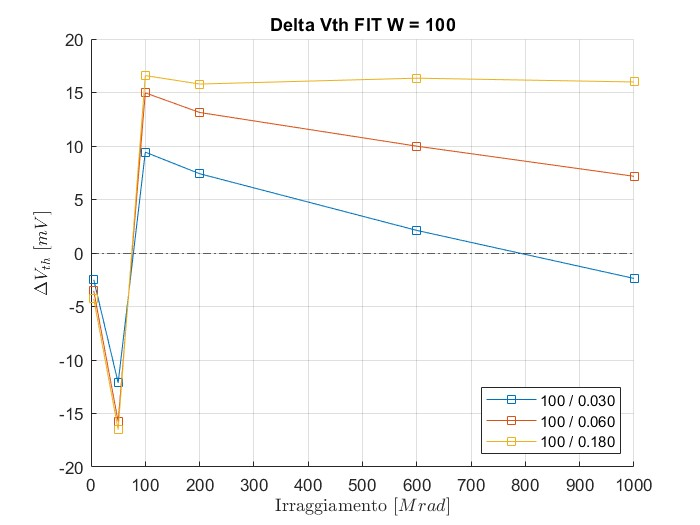
\includegraphics[width=0.49\textwidth]{./capitolo2/VTH/ELR/sovrapposizione-deltaVth-FIT-N100}
  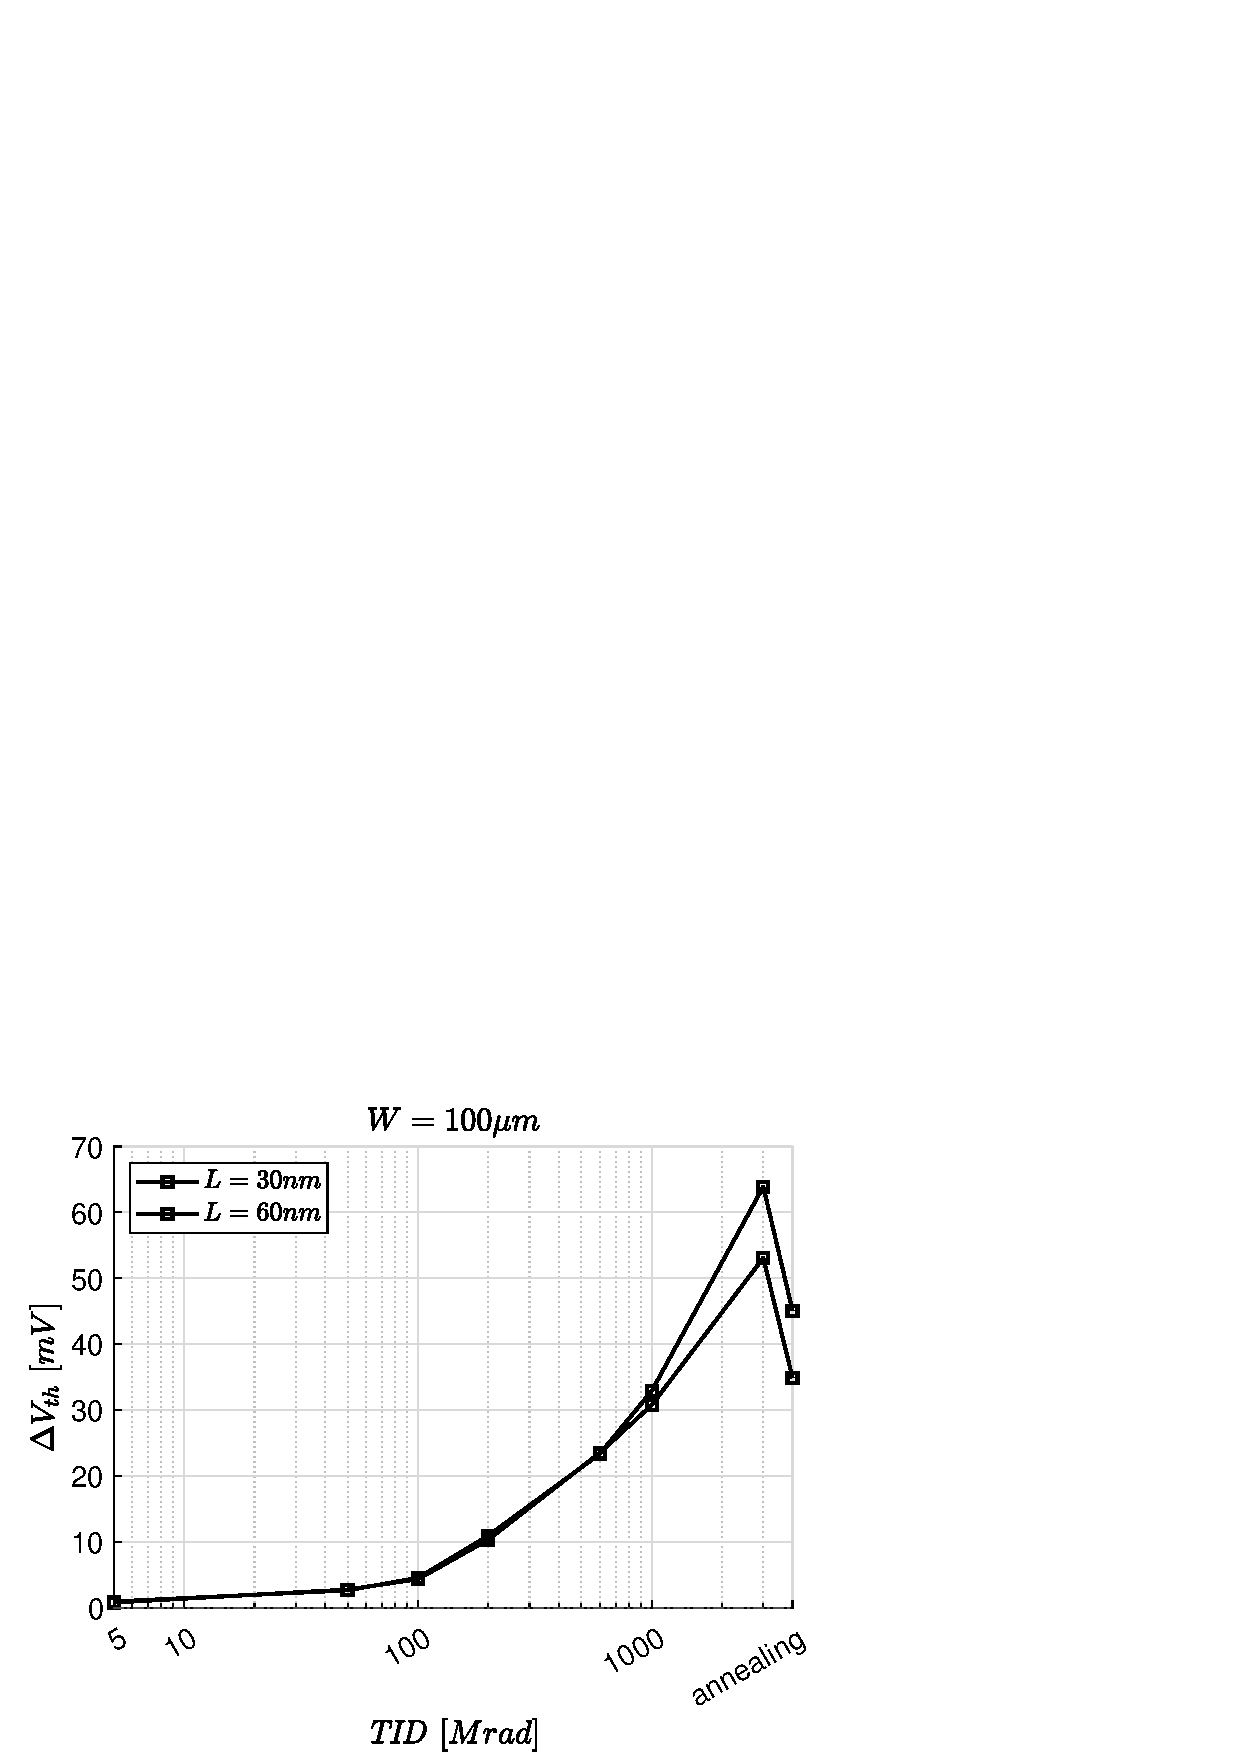
\includegraphics[width=0.49\textwidth]{./capitolo2/VTH/ELR/sovrapposizione-deltaVth-FIT-P100}
  % W = 200
  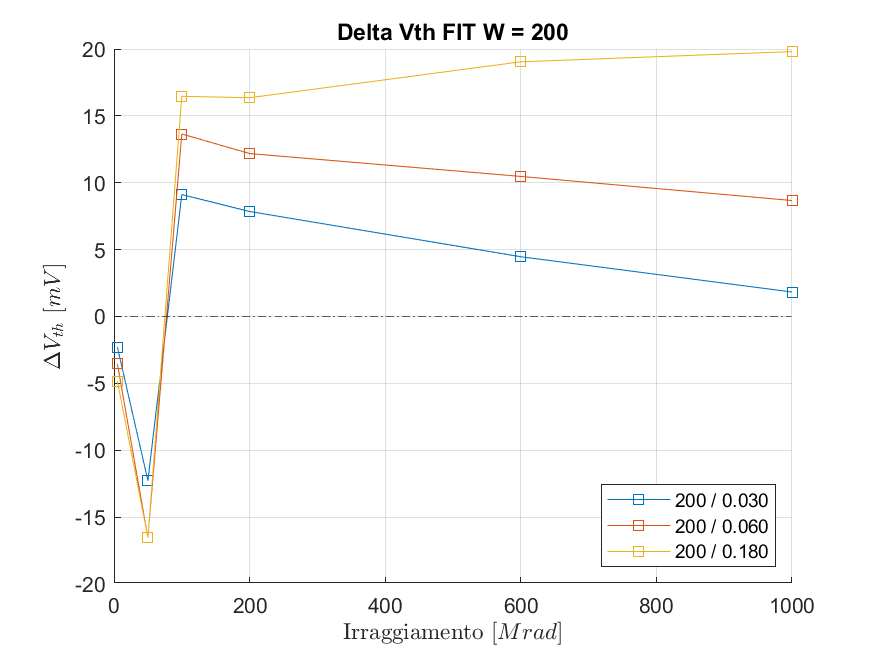
\includegraphics[width=0.49\textwidth]{./capitolo2/VTH/ELR/sovrapposizione-deltaVth-FIT-N200}
  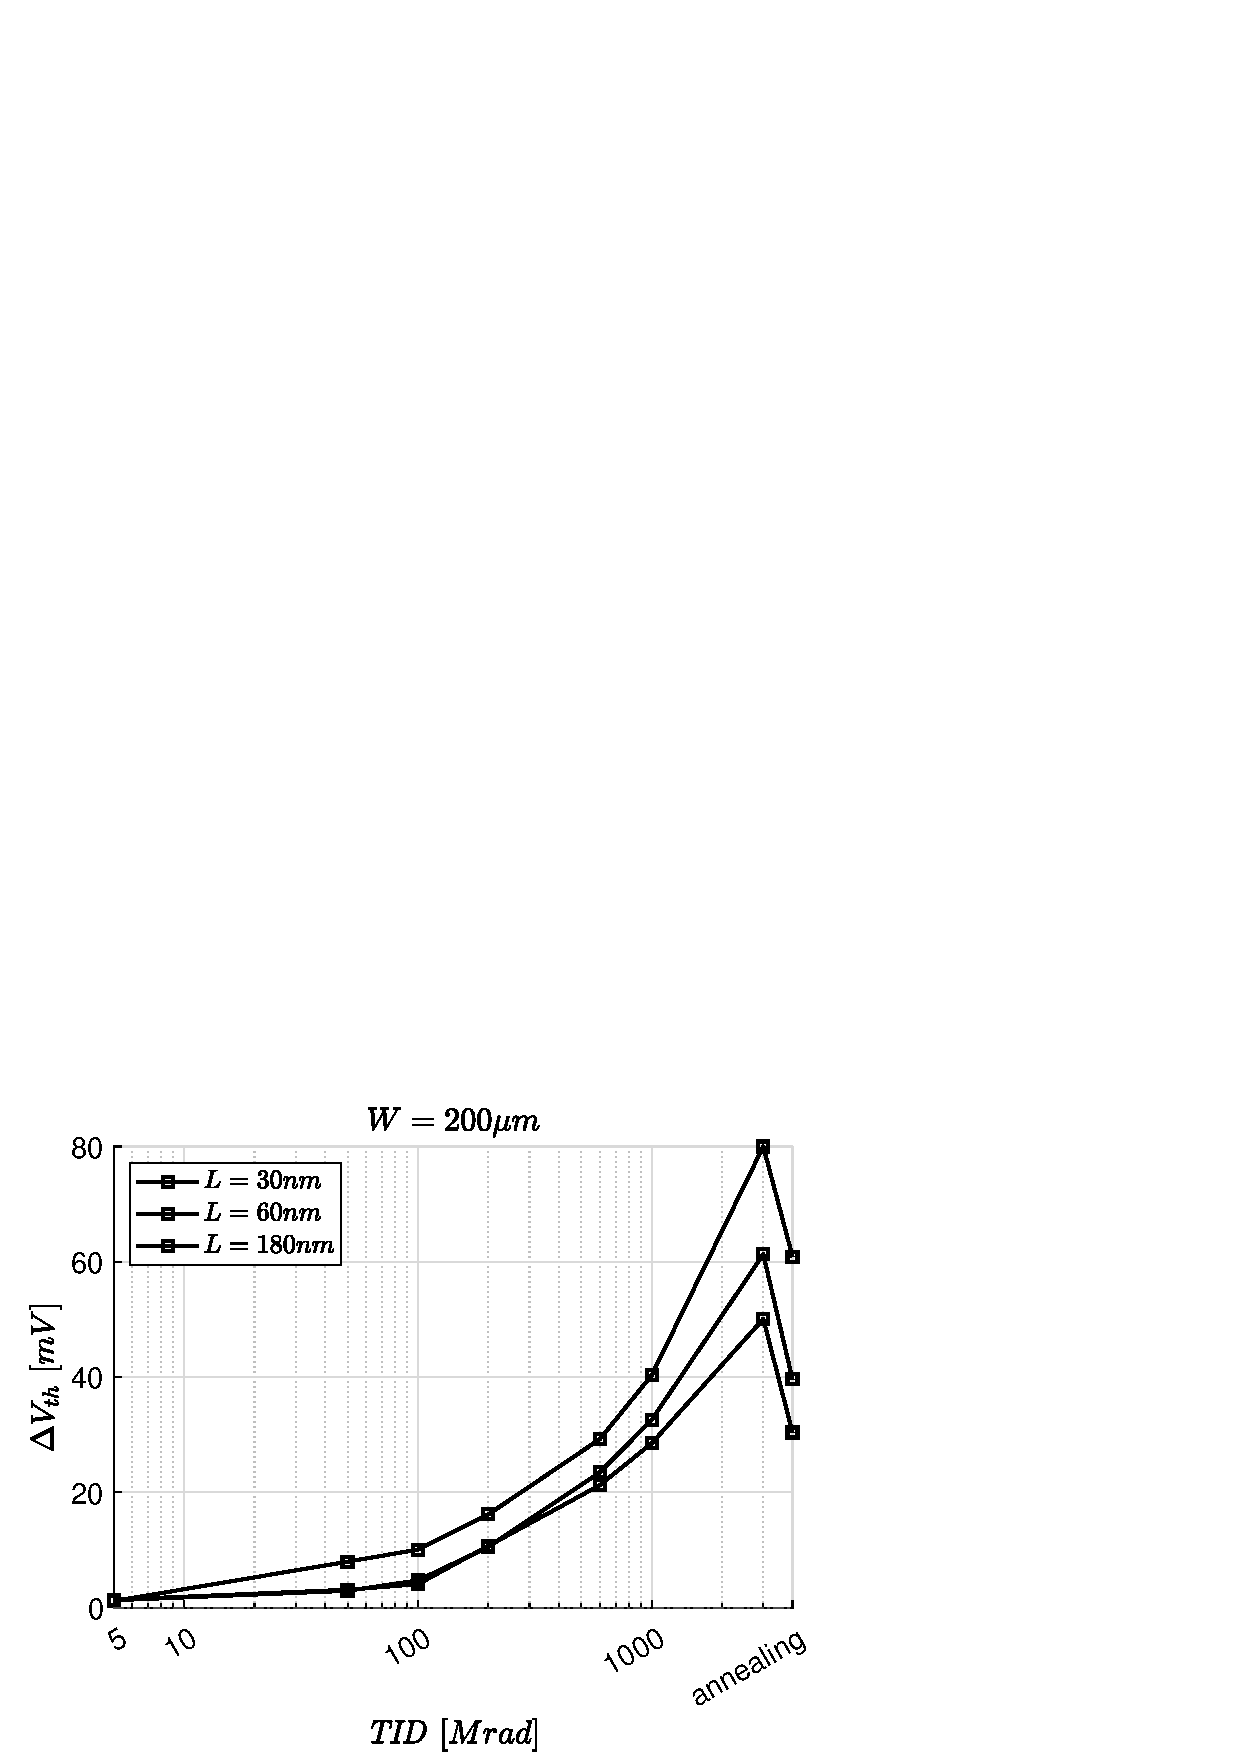
\includegraphics[width=0.49\textwidth]{./capitolo2/VTH/ELR/sovrapposizione-deltaVth-FIT-P200}
  % W = 600
  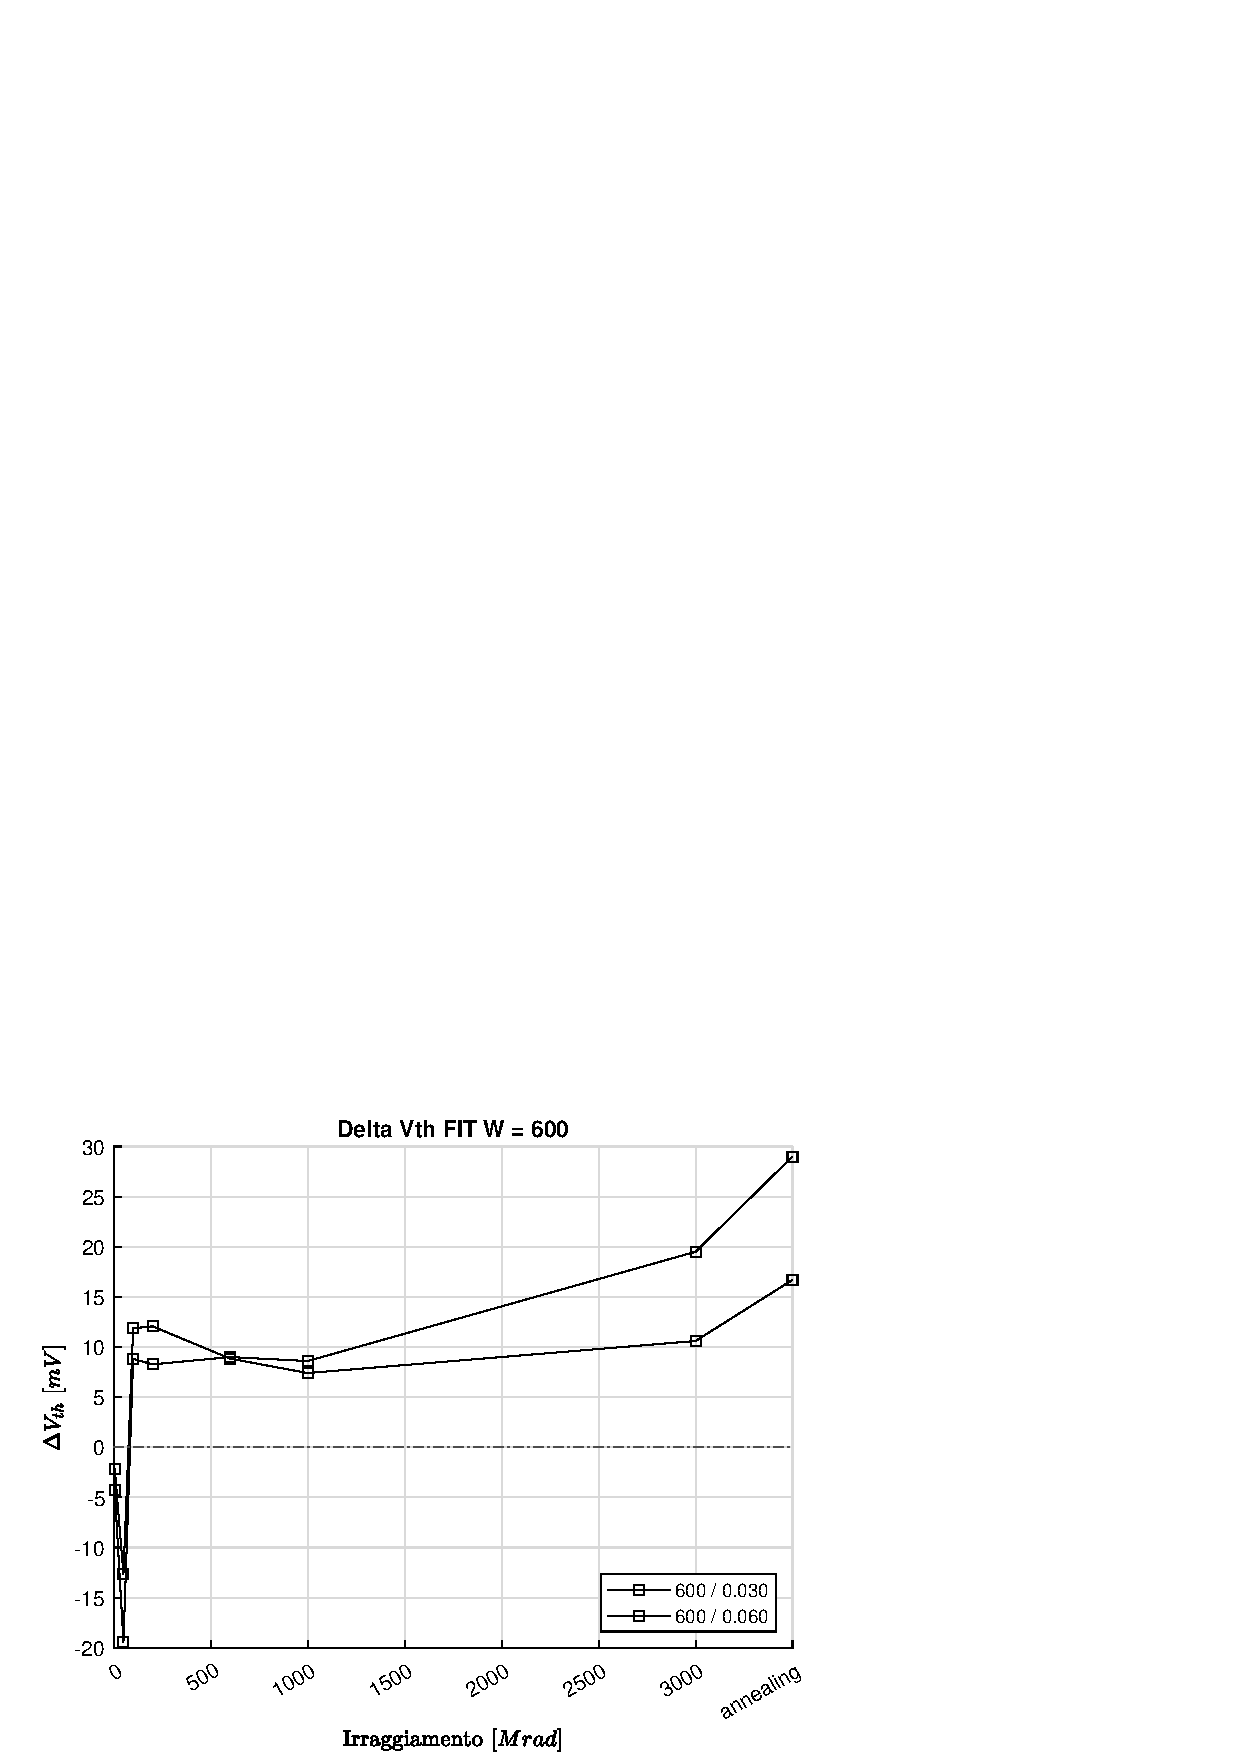
\includegraphics[width=0.49\textwidth]{./capitolo2/VTH/ELR/sovrapposizione-deltaVth-FIT-N600}
  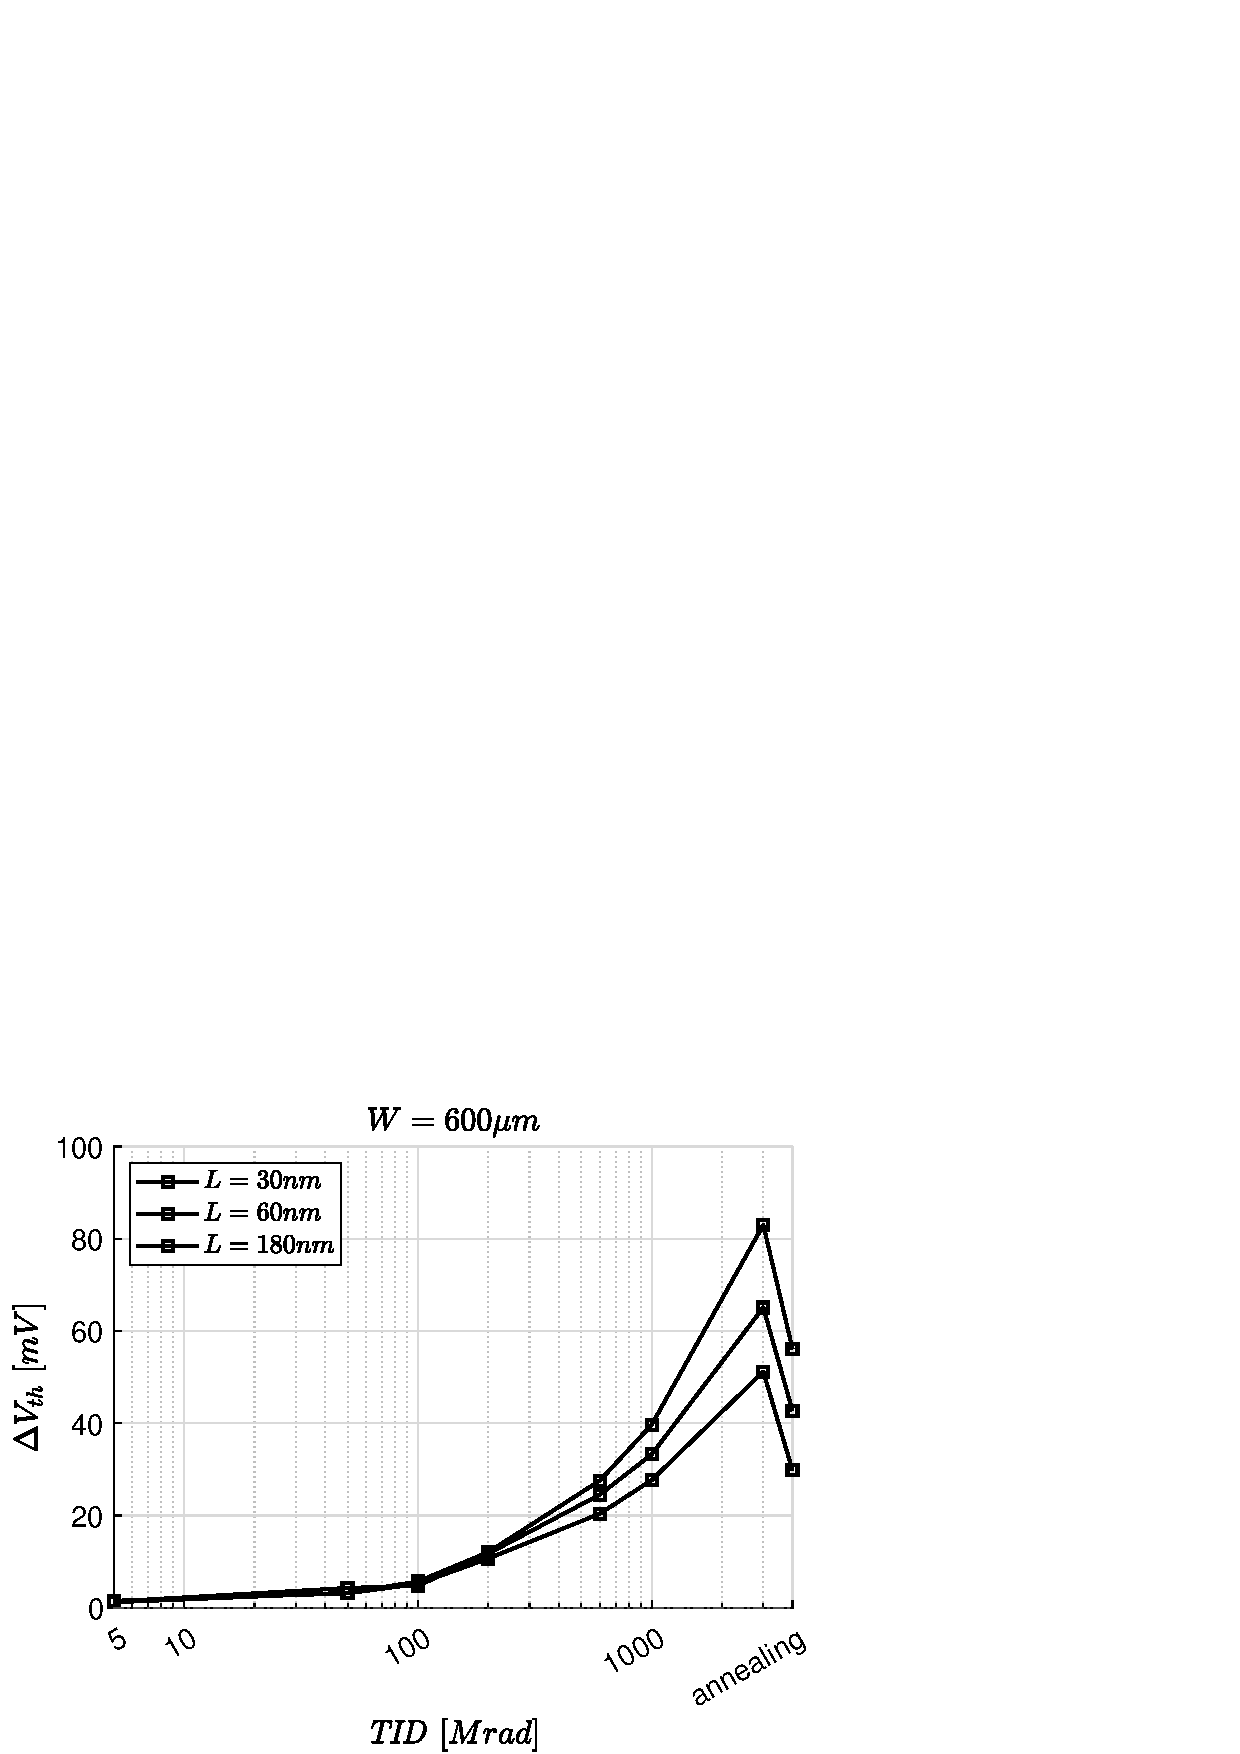
\includegraphics[width=0.49\textwidth]{./capitolo2/VTH/ELR/sovrapposizione-deltaVth-FIT-P600}
  \caption[Dati $\Delta V_{th}$ estratti con ELR]{Variazioni di $V_{th}$ dei dispositivi NMOS (a sinistra) PMOS (a destra) estratte con \emph{ELR} in funzione della dose assorbita. Ogni figura si riferisce a una larghezza di canale W differente.}
\end{figure}

\subsection[RM]{Ratio Method}
Il \emph{Ratio Method, RM} è stato sviluppato per far fronte alle problematicità dell'\emph{ELR}: è stato infatti dimostrato che questo metodo non è influenzato dalla degradazione della mobilità dei portatori di carica né dalle resistenze parassite\cite{art2}. Questo metodo si basa sull'assunzione che, a bassi valori di tensione di drain $V_{DS}$, il rapporto tra la corrente di drain $I_D$ e la radice quadrata della transconduttanza $g_m$ ($\frac{I_D}{\sqrt{g_m}}$) in funzione della tensione di gate $V_{GS}$ si comporti come una funzione lineare. La tensione di soglia $V_{th}$ coincide con il valore della tensione $V_{GS}$ a cui il fit lineare della funzione interseca l'asse delle ascisse.\\
Come detto, questo metodo supera alcuni limiti dei metodi descritti in precedenza, però presenta una problematicità non indifferente: tracciando il grafico di $\frac{I_D}{\sqrt{g_m}}$ in funzione di $V_{GS}$, questo non verifica appieno l'assunzione di linearità. Dunque non esiste un intervallo in cui il grafico è chiaramente linearizzabile e quindi la misura di $V_{th}$ non rispecchia del tutto il valore reale della tensione di soglia, ma è comunque una buona approssimazione, soprattutto se si considera il $\Delta V_{th}$ al crescere dell'irraggiamento.
Anche il questo caso, per ottenere il fit lineare più accurato possibile è stato usato lo stesso metodo esposto per l'\emph{ELR}.


\begin{figure}[h!]
  \centering
  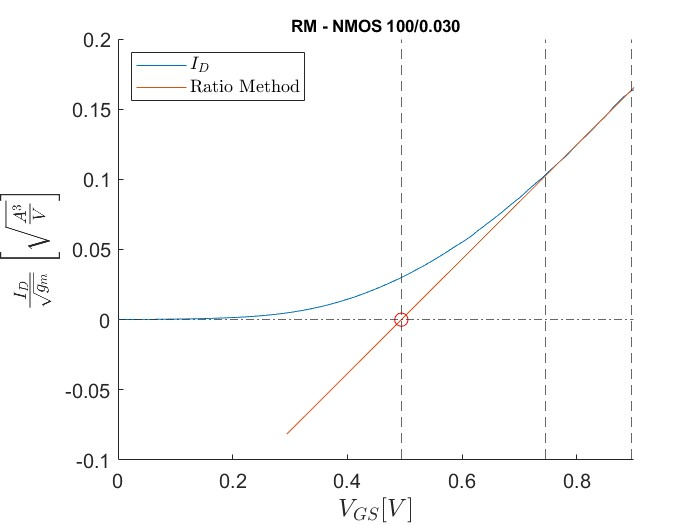
\includegraphics[width=0.49\textwidth]{./capitolo2/VTH/RM/RM-N4-100-30}
  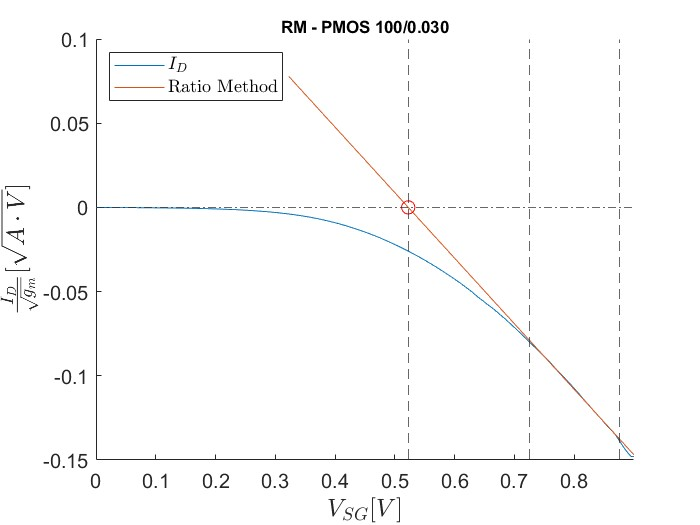
\includegraphics[width=0.49\textwidth]{./capitolo2/VTH/RM/RM-P1-100-30}
  \caption[Applicazione RM]{Fit lineare della caratteristica $\frac{I_D}{\sqrt{g_m}}-V_{GS}$ a $V_{DS}=150mV$ di un NMOS e di un PMOS di dimensioni 100-0.030}
\end{figure}



\begin{table}[H]
  \renewcommand{\arraystretch}{1.3}
  \resizebox{\textwidth}{!}{%
    \begin{tabular}{c c c c c c c c c c }
      \toprule
      \multirow{2}{*}{Dispositivo} & \multicolumn{9}{c}{$V_{th} [mV] $}                                                                                          \\
      \cmidrule{2-10}
                                   & pre                                & $5Mrad$ & $50Mrad$ & $100Mrad$ & $200Mrad$ & $600Mrad$ & $1Grad$ & $3Grad$ & annealing \\
      \midrule
      100 - 0.030                  & 494.2                              & 490.9   & 476.2    & 449.9     & 447.5     & 478.7     & 478.4   & 444.0   & 489.9     \\
      \hline
      100 - 0.060                  & 485.6                              & 481.8   & 470.9    & 502.5     & 499.4     & 500.3     & 499.4   & 506.0   & 506.9     \\
      \hline
      100 - 0.180                  & 529.4                              & 527.8   & 503.8    & 541.0     & 541.9     & 541.4     & 540.9   & 545.8   & 550.8     \\
      \hline
      200 - 0.030                  & 485.2                              & 497.4   & 483.1    & 486.8     & 496.7     & 504.1     & 497.3   & 500.3   & 499.0     \\
      \hline
      200 - 0.060                  & 499.8                              & 482.9   & 467.2    & 499.6     & 498.9     & 503.1     & 514.1   & 513.6   & 518.1     \\
      \hline
      200 - 0.180                  & 523.4                              & 515.8   & 507.5    & 542.1     & 538.6     & 544.1     & 546.2   & 506.6   & 555.1     \\
      \hline
      600 - 0.060                  & 514.9                              & 507.4   & 504.9    & 517.3     & 521.4     & 521.2     & 514.3   & 512.8   & 526.5     \\
      \hline
      600 - 0.180                  & 539.0                              & 537.0   & 525.9    & 546.6     & 546.2     & 545.6     & 546.1   & 550.2   & 557.4     \\
      \bottomrule
    \end{tabular}%
  }
  \caption[$V_{th}$ dei dispositivi NMOS estratte con RM]{$V_{th}$ dei dispositivi NMOS estratte con \emph{RM}}
  \label{tab:VthRMN}
\end{table}


\begin{table}[H]
  \renewcommand{\arraystretch}{1.3}
  \resizebox{\textwidth}{!}{%
    \begin{tabular}{c c c c c c c c c c }
      \toprule
      \multirow{2}{*}{Dispositivo} & \multicolumn{9}{c}{$|V_{th}| [mV] $}                                                                                          \\
      \cmidrule{2-10}
                                   & pre                                & $5Mrad$ & $50Mrad$ & $100Mrad$ & $200Mrad$ & $600Mrad$ & $1Grad$ & $3Grad$ & annealing \\
      \midrule
      100 - 0.030                  & 522.3                              & 529.8   & 530.7    & 532.2     & 533.3     & 544.4     & 547.3   & 520.9   & 553.1     \\
      \hline
      100 - 0.060                  & 543.6                              & 543.3   & 541.8    & 545.4     & 548.9     & 528.1     & 541.6   & 581.5   & 560.3     \\
      \hline
      200 - 0.030                  & 525.2                              & 520.5   & 527.4    & 542.2     & 544.8     & 551.1     & 554.7   & 554.0   & 553.5     \\
      \hline
      200 - 0.060                  & 547.9                              & 540.5   & 549.1    & 550.6     & 555.7     & 563.1     & 568.3   & 579.3   & 571.1     \\
      \hline
      200 - 0.180                  & 551.1                              & 553.1   & 538.3    & 538.0     & 545.0     & 568.8     & 576.8   & 599.7   & 587.5     \\
      \hline
      600 - 0.030                  & 527.8                              & 539.9   & 537.3    & 540.2     & 539.9     & 550.8     & 555.2   & 567.0   & 556.5     \\
      \hline
      600 - 0.060                  & 557.2                              & 552.2   & 558.5    & 559.7     & 558.7     & 567.6     & 576.7   & 589.6   & 575.2     \\
      \hline
      600 - 0.180                  & 555.2                              & 559.3   & 556.9    & 559.4     & 559.7     & 574.3     & 581.3   & 603.4   & 582.1     \\
      \bottomrule
    \end{tabular}%
  }
  \caption[$|V_{th}|$ dei dispositivi PMOS estratte con RM]{$|V_{th}|$ dei dispositivi PMOS estratte con \emph{RM}}
  \label{tab:VthRMP}
\end{table}


\begin{table}[H]
  \renewcommand{\arraystretch}{1.3}
  \resizebox{\textwidth}{!}{%
    \begin{tabular}{c c c c c c c c c}
      \toprule
      \multirow{2}{*}{Dispositivo} & \multicolumn{8}{c}{$\Delta V_{th} [mV] $}                                                                                \\
      \cmidrule{2-9}
                                   & $5Mrad$                                   & $50Mrad$ & $100Mrad$ & $200Mrad$ & $600Mrad$ & $1Grad$ & $3Grad$ & annealing \\
      \midrule
      100 - 0.030                  & -3.3                                      & -18.0    & -44.3     & -46.7     & -15.4     & -15.8   & -50.2   & -4.3      \\
      \hline
      100 - 0.060                  & -3.9                                      & -14.7    & 16.8      & 13.8      & 14.7      & 13.8    & 20.4    & 21.3      \\
      \hline
      100 - 0.180                  & -1.6                                      & -25.6    & 11.6      & 12.6      & 12.0      & 11.5    & 16.4    & 21.4      \\
      \hline
      200 - 0.030                  & 12.2                                      & -2.1     & 1.7       & 11.5      & 19.0      & 12.1    & 15.1    & 13.8      \\
      \hline
      200 - 0.060                  & -16.9                                     & -32.5    & -0.2      & -0.9      & 3.3       & 14.3    & 13.8    & 18.3      \\
      \hline
      200 - 0.180                  & -7.6                                      & -15.9    & 18.7      & 15.2      & 20.7      & 22.8    & -16.8   & 31.7      \\
      \hline
      600 - 0.060                  & -7.5                                      & -9.9     & 2.4       & 6.5       & 6.3       & -0.6    & -2.1    & 11.6      \\
      \hline
      600 - 0.180                  & -1.9                                      & -13.0    & 7.6       & 7.2       & 6.7       & 7.1     & 11.2    & 18.4      \\
      \bottomrule
    \end{tabular}%
  }
  \caption[$\Delta V_{th}$ dei dispositivi NMOS estratte con RM]{$\Delta V_{th}$ dei dispositivi NMOS estratte con \emph{RM}}
  \label{tab:deltaVthRMN}
\end{table}


\begin{table}[H]
  \renewcommand{\arraystretch}{1.3}
  \resizebox{\textwidth}{!}{%
    \begin{tabular}{c c c c c c c c c}
      \toprule
      \multirow{2}{*}{Dispositivo} & \multicolumn{8}{c}{$\Delta V_{th} [mV] $}                                                                                \\
      \cmidrule{2-9}
                                   & $5Mrad$                                   & $50Mrad$ & $100Mrad$ & $200Mrad$ & $600Mrad$ & $1Grad$ & $3Grad$ & annealing \\
      \midrule
      100 - 0.030                  & 7.5                                       & 8.4      & 9.9       & 11.0      & 22.1      & 25.1    & -1.4    & 30.8      \\
      \hline
      100 - 0.060                  & -0.3                                      & -1.8     & 1.8       & 11.0      & -15.5     & -2.0    & 37.9    & 16.7      \\
      \hline
      200 - 0.030                  & -4.7                                      & 2.2      & 17.0      & 19.6      & 25.9      & 29.5    & 28.8    & 28.3      \\
      \hline
      200 - 0.060                  & -7.5                                      & 1.1      & 2.6       & 7.7       & 15.2      & 20.3    & 31.4    & 23.2      \\
      \hline
      200 - 0.180                  & 2.0                                       & -12.7    & -13.1     & -6.1      & 17.8      & 25.7    & 48.6    & 36.4      \\
      \hline
      600 - 0.030                  & 12.1                                      & 9.5      & 12.4      & 12.1      & 23.0      & 27.5    & 39.2    & 28.7      \\
      \hline
      600 - 0.060                  & 12.1                                      & 1.3      & 2.5       & 12.1      & 10.4      & 19.5    & 32.4    & 18.0      \\
      \hline
      600 - 0.180                  & -4.6                                      & 1.8      & 4.3       & 4.5       & 19.2      & 26.1    & 48.2    & 26.9      \\
      \bottomrule
    \end{tabular}%
  }
  \caption[$\Delta V_{th}$ dei dispositivi PMOS estratte con RM]{$\Delta V_{th}$ dei dispositivi PMOS estratte con \emph{RM}}
  \label{tab:deltaVthRMP}
\end{table}

\begin{figure}[H]
  \centering
  % W = 100 
  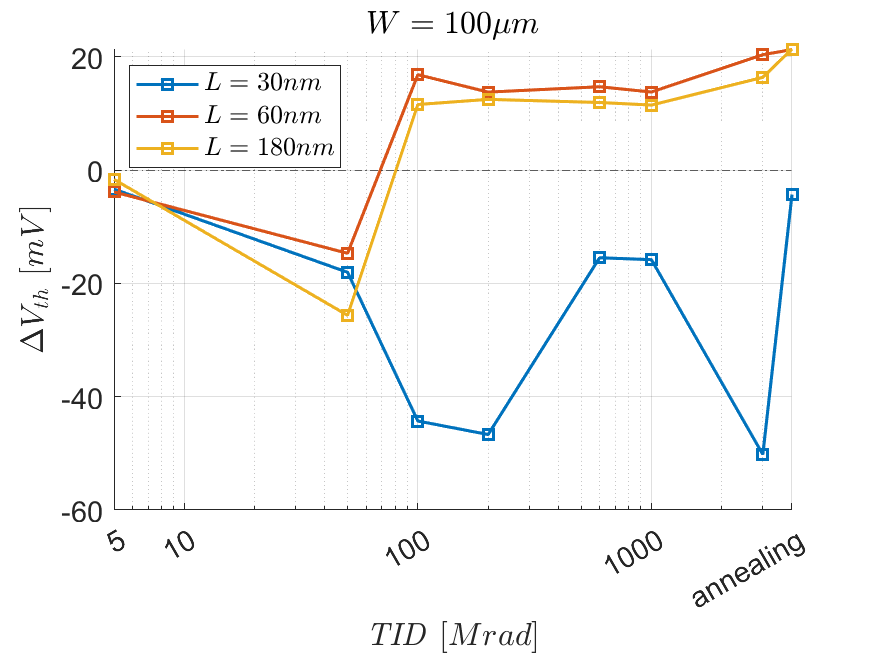
\includegraphics[width=0.49\textwidth]{./capitolo2/VTH/RM/sovrapposizione-deltaVth-RM-N100}
  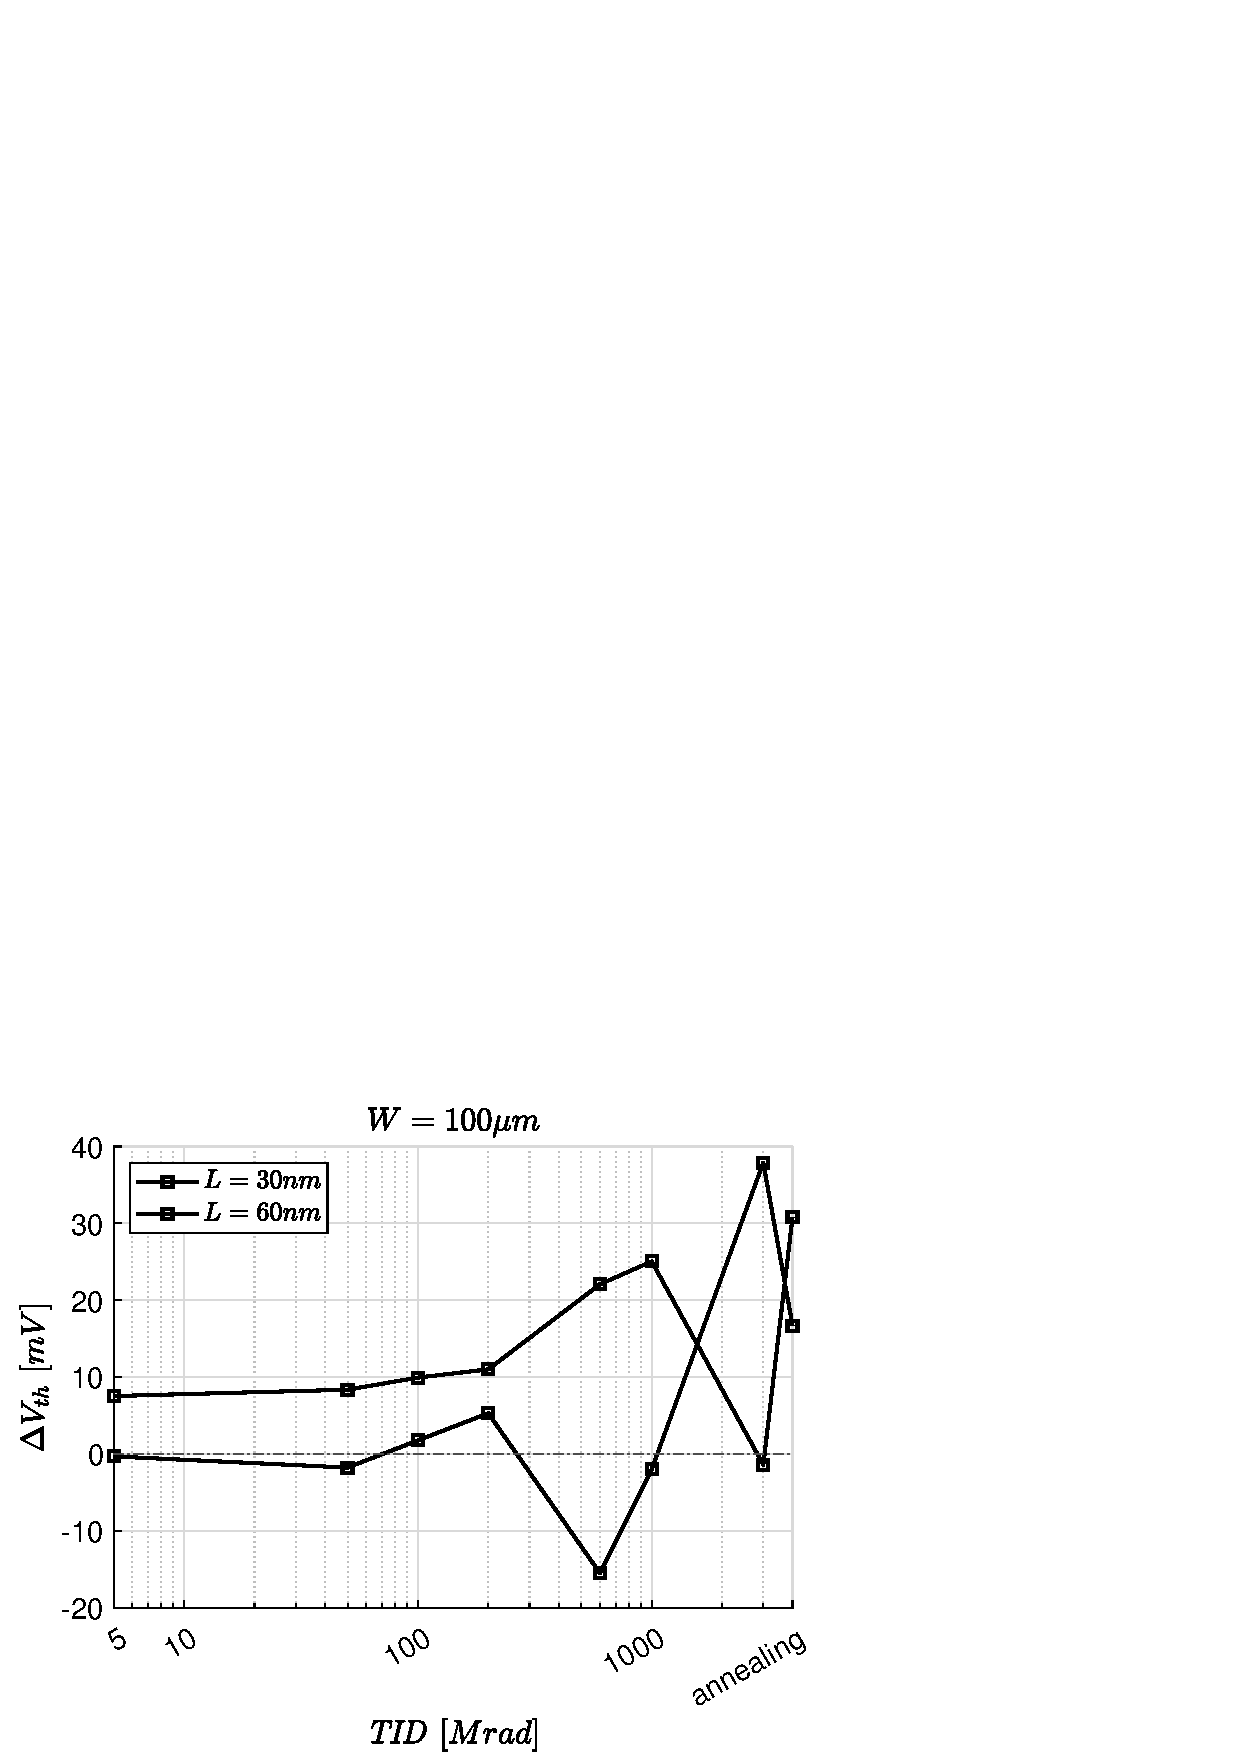
\includegraphics[width=0.49\textwidth]{./capitolo2/VTH/RM/sovrapposizione-deltaVth-RM-P100}
  % W = 200
  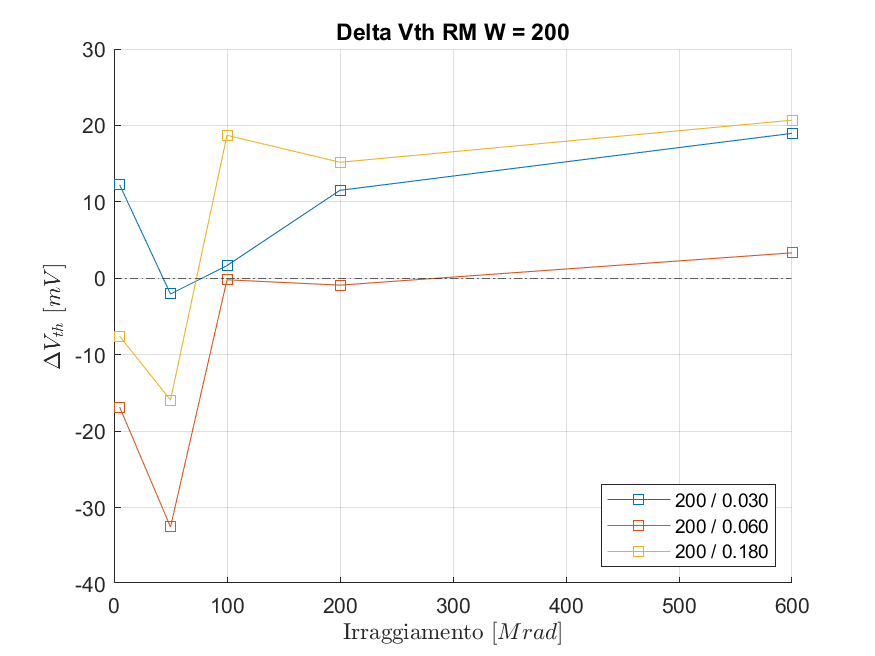
\includegraphics[width=0.49\textwidth]{./capitolo2/VTH/RM/sovrapposizione-deltaVth-RM-N200}
  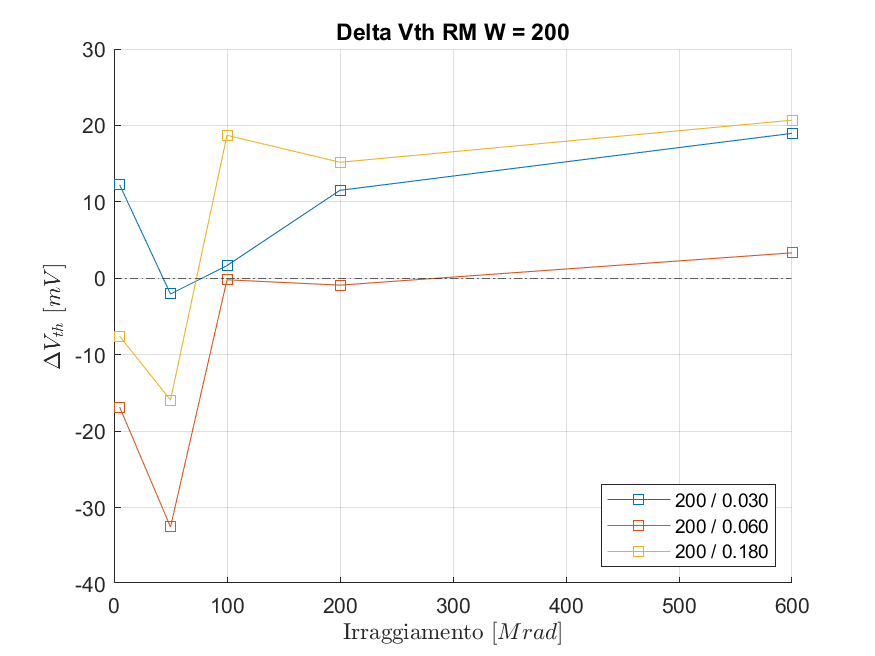
\includegraphics[width=0.49\textwidth]{./capitolo2/VTH/RM/sovrapposizione-deltaVth-RM-P200}
  % W = 600
  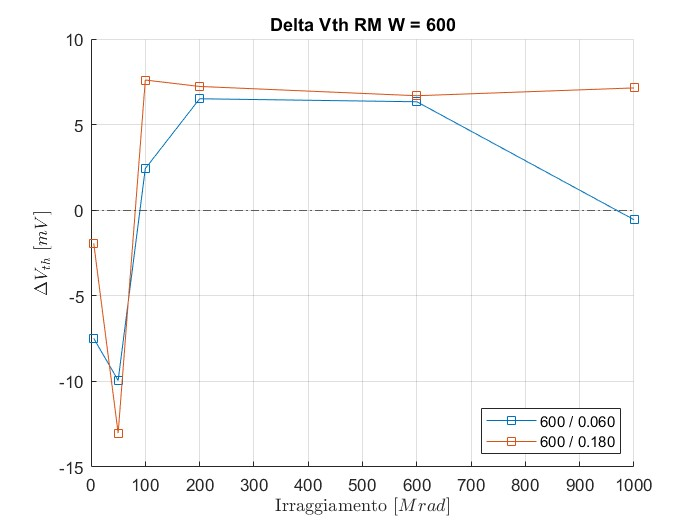
\includegraphics[width=0.49\textwidth]{./capitolo2/VTH/RM/sovrapposizione-deltaVth-RM-N600}
  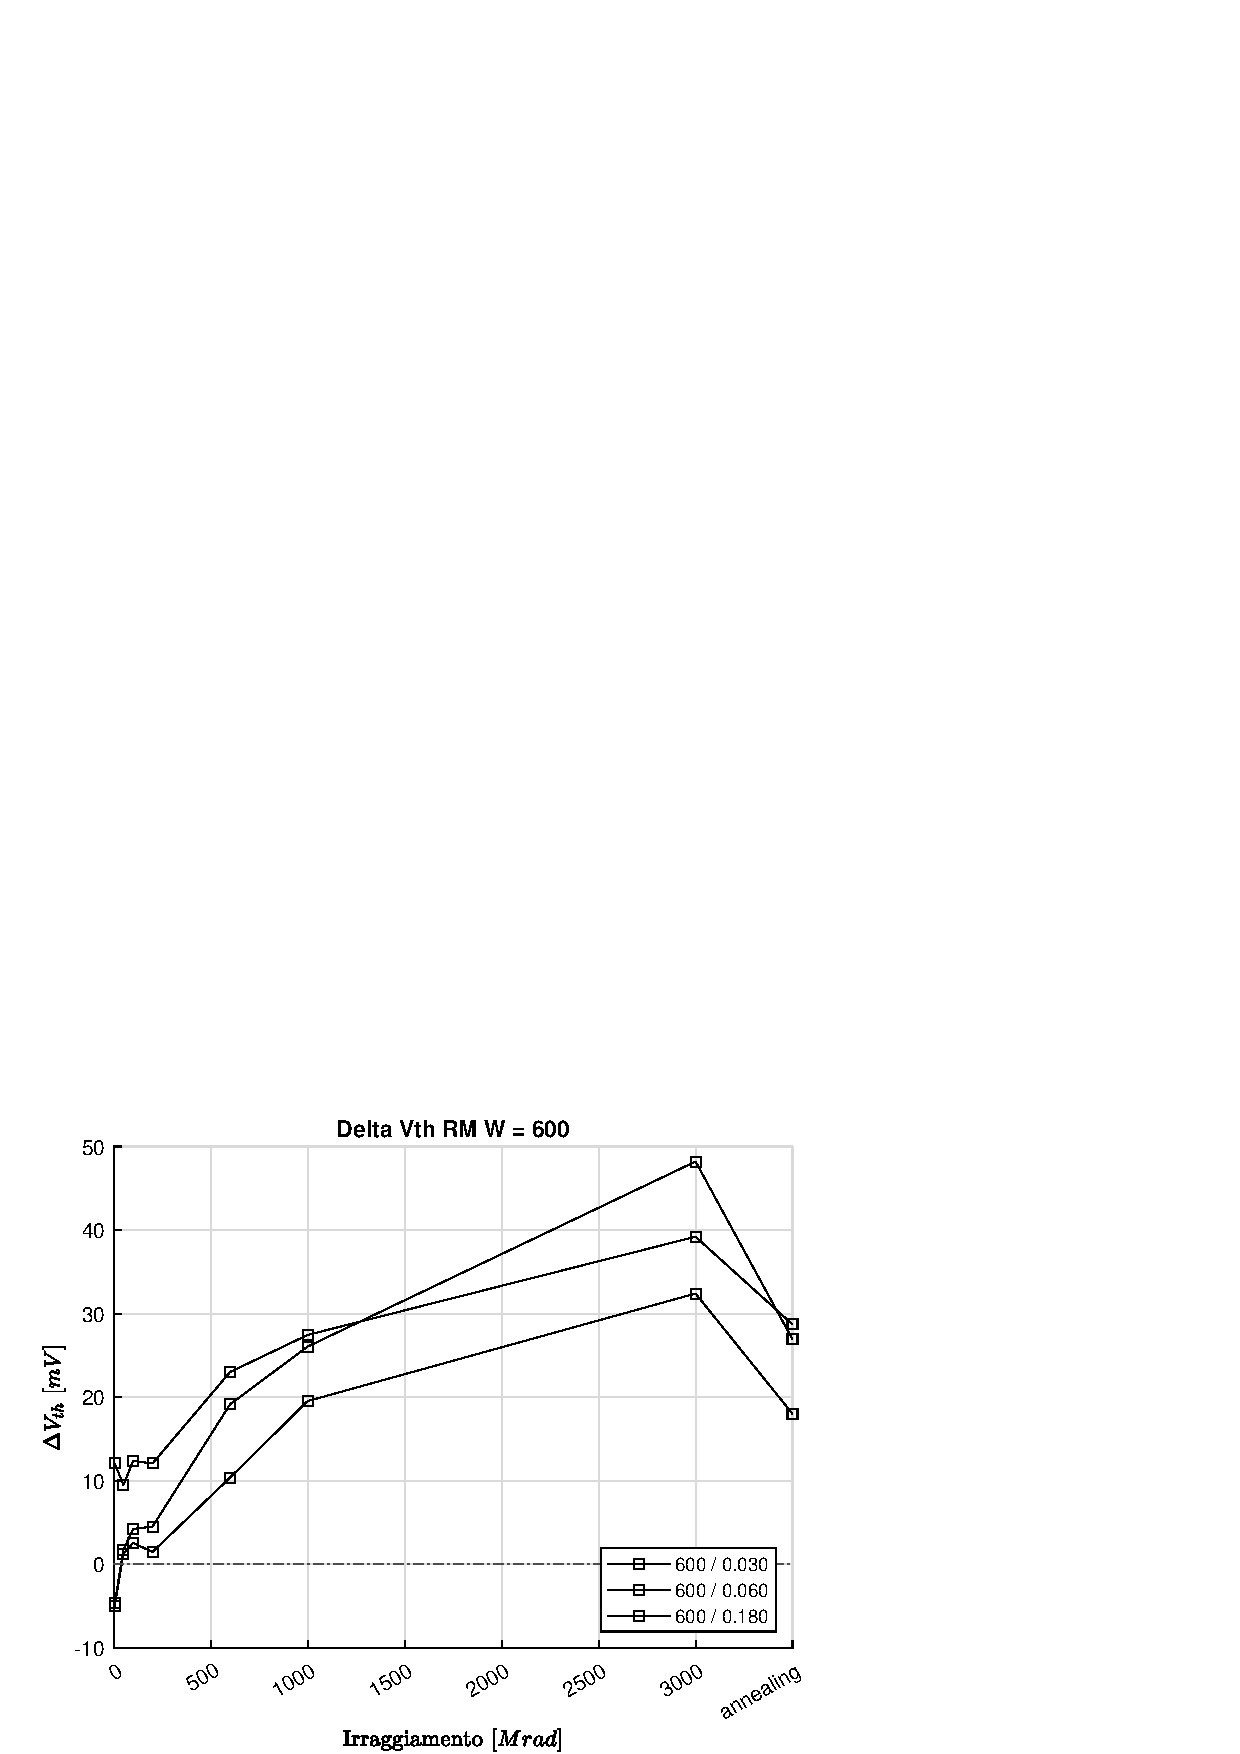
\includegraphics[width=0.49\textwidth]{./capitolo2/VTH/RM/sovrapposizione-deltaVth-RM-P600}
  \caption[Dati $\Delta V_{th}$ estratti con RM]{Variazioni di $V_{th}$ dei dispositivi NMOS (a sinistra) PMOS (a destra) estratte con \emph{RM} in funzione della dose assorbita. Ogni figura si riferisce a una larghezza di canale W differente.}

\end{figure}


\subsection{Riepilogo}
Per concludere questa sezione si vuole fare un confronto tra i diversi metodi per trovare quello (o quelli) più aderente alla teoria sugli effetti delle radiazioni ionizzanti sui dispositivi MOSFET descritta nella sezione \ref{cap1:ionizzazione}.
Si è scelto di fare i confronti, con dispositivo a larghezza $100\mu m$ e lunghezza $30nm$ sia per i transistori MOSFET a canale N che a canale P  
